\documentclass[a4paper]{book}
\usepackage{url, graphicx, wrapfig, hyperref, ifthen, enumitem, makeidx, microtype, booktabs, caption}
\usepackage{currfile}
\usepackage[numbib, numindex]{tocbibind}
\usepackage[superscript]{cite}
\makeindex
\setcounter{secnumdepth}{0}
\title{The C. F. Barker Archives}
\author{\url{http://samwilson.github.io/cfb}}

\usepackage{relsize,etoolbox}% http://ctan.org/pkg/{relsize,etoolbox}
\AtBeginEnvironment{quotation}{\smaller}% Step font down one size relative to current font.

\hypersetup{
  colorlinks = true,  % Colours links instead of ugly boxes
  urlcolor   = blue,  % Colour for external hyperlinks
  linkcolor  = black, % Colour of internal links
  citecolor  = black  % Colour of citations
}

% ---- \biohead{Full Name}{Caption for photo.}
% \biohead{}{}
\newcommand{\biohead}[2]{%
	\section{#1}\label{\currfilebase}%
	\ifthenelse { \equal {#2} {} }%
	{} % If #2 is empty, do nothing
	{ % Otherwise, do the figure
	\begin{wrapfigure}{l}{0.25\textwidth}%
		\vspace{-12pt}%
		\centering
		\includegraphics[width=0.8\linewidth]{photos/\currfilebase} \\
		{\footnotesize #2}%
		\label{fig:\currfilebase}
		\vspace{-12pt}%
	\end{wrapfigure}%
	}%
}

% ---- \p{label} results in e.g. "p. 3"
\newcommand{\p}[1]{p.~\pageref{#1}}

% ---- \idx{}
\newcommand{\idx}[1]{#1\index{#1}}


\begin{document}
\maketitle
\tableofcontents

\chapter{People}

% Generation 1
\biohead{Ralph Munday Denton-Barker}{7 July 1942.}

Ralph Denton-Barker was born on 17 July 1916 in Birkenhead to James Denton Barker (\p{James_Denton_Barker}) and
Kathleen Munday (\p{Kathleen_Munday}). He had two siblings: Bertram Mead Denton Barker (\p{Bertram_Mead_Denton_Barker}) and Virginia Kathleen Denton Barker (\p{Virginia_Kathleen_Denton_Barker}) \cite{BMDIndex_RalphMundayDentonBarker_birth}.

Ralph was educated at Cheam and Felsted School, and Birkenhead School. He joined the Alliance Insurance Company to train as an actuary, but left the company on joining the army at the beginning of the war. He served as a Private soldier throughout the war. 

He married Joan Nyria Powell (nee Hancox)(\p{Joan_Nyria_Hancox}) on 28 June 1947 at the Register Office, Edmonton, Middlesex.\cite{MarriageCertRalphDentonBarkerJoanNyriaPowell} and they had one daughter, Julia.

After demobilisation, he trained as a primary school teacher, and worked as a teacher at Kimbolton School,  Bedfordshire (living at the Old Schoolhouse in Pertenhall), next in  Worcestershire (living at Dove Cottage near Great Witley and teaching at Arley Kings Primary School) and then in Cornwall (firstly living at The Barn, Portloe) where he taught at Mevagissey Primary School.  They  bought Kerrow Farm in West Penwith in 1965 where they farmed (dairy and beef cattle) for five years. 
He retired from teaching in 1970, and they then moved to \idx{Menorca} where they had a small holding (known as a finca) outside Alayor. Ralph continued to raise a few cattle and also taught English to people in Alayor.  They then moved to C'an Amoros, outside Pollensa in Mallorca where Ralph had a few cows and a large citrus orchard.

They moved to Australia in 1978, travelling on a Russian ship (via Sri Lanka, arriving on March 17th), and after a year in Western Australia (living on Lapko's Farm, \idx{Denmark}) they settled in \idx{Tasmania} at Riverside Cottage, Upper Scamander, on the east coast. There they kept a few cattle and some goats and developed a large organic garden.

He died on 4 November 1990\cite{RMDBarkerDeath, RalphDeathCert} at home in Upper Scamander, and was buried on 6 November 1990 at St Helens Cemetery, Tasmania.

\begin{figure}
\centering
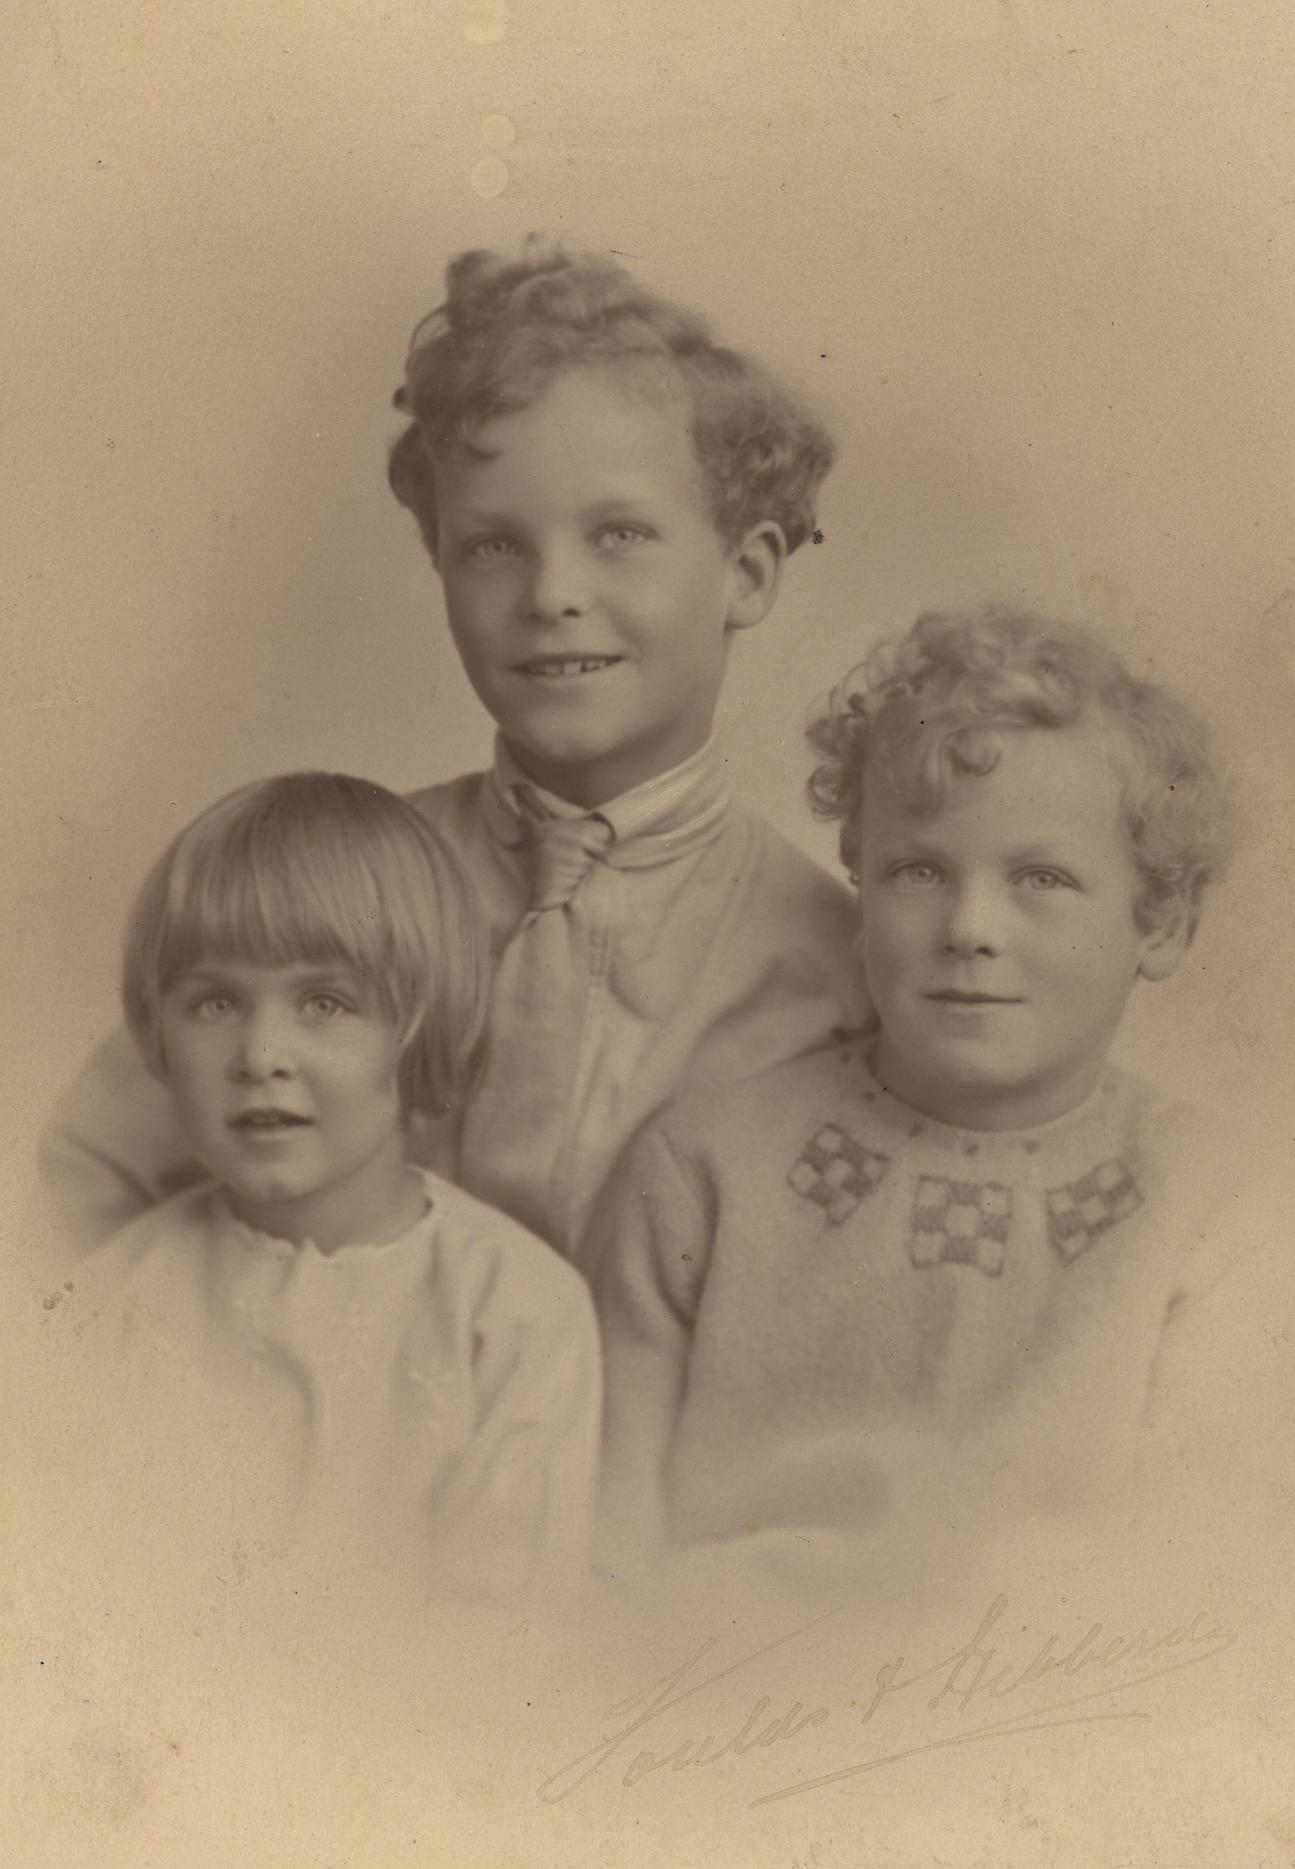
\includegraphics{photos/Mead_Ralph_Virginia_Nov_1922.png}
\caption{Mead, Ralph, and Virginia in November 1922.}
\end{figure}

\biohead{Joan Nyria Hancox}{Joan_Nyria_Hancox}{Late 1950s in Great Witley.\cite{FlickrNyria}}  

Nyria Denton-Barker (n\'{e}e Hancox)} (23 February 1918 -- 15 October 2004) was born in Bebington, Cheshire and was the only daughter of Richard James Hancox (1873--1956) and Marian Gilmour Croskery (1879--1970)[Nyriabirthcert].  She had one brother, Eric Geoffrey West Hancox (1911--1937).  They lived at 8 Thorburn Road, Rock Ferry and she was christened on 7 April 1918 [Nyria christening]
From the age of 6,  she attended Howell's School, Llandaff (in the Vale of Glamorgan, Wales [Nyria School].

In the mid-thirties she studied nursing at Guy's Hospital (enrolling under the approved age at the time),  where she was working  as a Sister on the children's ward at the beginning of the war until they were evacuated out of London. She then married Geoffrey Powell;  they lived in north London and had one son, David Powell (born in 1942).  
During the war she met Ralph Munday Denton-Barker and after divorcing her first husband, they married on 28 June, 1947 [Nyria marriage cert].  
They moved to Pertenhall, Bedfordshire in 1948 and had one daughter, Julia (born in 1949).  In 1954 they moved to Dove Cottage, Great Witley, Worcestershire and Nyria had a very large garden, producing most of the family vegetables and fruit. She taught pottery to deaf children while living there.  In 1960 they moved to The Barn, Portloe, Cornwall and Nyria was very involved in community activities in the area, and also was a keen choir member.  They had a holiday house near Zennor, and their love of the area led them to buy Kerrow Farm, West Penwith, Cornwall in 1965,  and she became a very active farmer for a few years as well as being engaged in the local arts community; she was an accomplished water colourist and potter.
In 1970, they left Cornwall and  bought a smallholding called Casa Din-Ding, near Alayor, Menorca and she enjoyed the gardening in  a new climate and challenge of living in a different country;  after a few years there, they moved to Mallorca and lived at Ca'an Amoros, near Pollensa.  
In 1978 they sold most of their belongings and went to Australia by ship arriving in Fremantle on March 17th.  For the first year they lived at Lapkos Farm, Denmark, Western Australia, and then in 1979 they drove overland and went to live in Tasmania at Riverside Cottage, Upper Scamander. They had 7 acres of land and developed a large and productive garden. Nyria was instrumental in setting up the Neighbourhood House in St Helens and was very involved in the east coast community.  She and Ralph also enjoyed many camping trips around the island and also northern New South Wales where they spent time in various intentional communities. 

She lived alone at Riverside Cottage after Ralph's death in 1990, until having a cerebral aneurysm in December 2000;  she then needed more care and lived at Medea Park, St Helens, but she still managed to maintain involvement and interest in her community activities.  She  died on 15 October 2004 in St Helens. Tasmania.

\section{Virginia Kathleen Denton Barker}\label{Virginia_Kathleen_Denton_Barker}

Virginia Kathleen Denton Barker (1919--2006) was born in Birkenhead, and educated at the Birkenhead High school for Girls (1924--37), and University College, London (1937--41). She graduated in 1941 in Anthropology, Economics and Psychology (II.i). From 1941 to 1945 she worked for the Wartime Social Survey (Ministry of Information) first as an interviewer and later in charge of the Survey of Sickness. From 1945--48 she worked with the Secretariat of the Royal Commission on Population. She was offered a place to read medicine at St. Bartholomew's Hospital in the first year that the Hospital admitted women as medical students. However, she did not take up this offer, instead marrying Eugene Grebenik on 28th December 1946. From 1948--60 she was engaged with domestic life and child rearing (three children: Michael, Peter and Catherine). From 1960--69 she worked as a part-time lecturer in Education at the Yorkshire College of Housecraft, which was to become Leeds Polytechnic and later, Leeds Metropolitan University. From 1973--84 she worked as Psychiatric Social worker at Holloway Sanatorium, Virginia Water, Surrey. On retiring in 1978 she was active in forming the Runnymede Mental Health Association, which provided care for patients discharged from Holloway and for other patients who were living in the Community. She was also President of the RMHA. A new wing for day respite centre was named after her. \cite{VirginiaDocs} Went to Perth (Western Australia) in 1982 to visit family.

\biohead{Eugenia Grebenik}{}{c.~1980}\index{Grebby}\index{Grebenik, Eugenia}

\emph{The following is Grebby's entry in Wikipedia:\footnote{\url{http://en.wikipedia.org/wiki/Eugene_Grebenik}}}

Eugene Grebenik CB, known as ``Grebby'' (20 July 1919, Kiev -- 14 October 2001, Oxford) was a central figure in the development of demography in Britain and the first director of the British Civil Service College.

Grebenik was the only son and elder child of Schulim Grebenik (1887--1972), estate agent, and his wife, Lea Helene, n\'{e}e Lopatizkaya (1894--1985), a qualified lawyer, both Jewish. His birth was not registered with the Ukrainian government because his mother didn't want him to be naturalised and thought that this was mandatory.\cite{PopStudies} He had a sister, Renata Rosalie. The family moved to Danzig in 1920, then to Berlin, and finally, after the rise of Adolf Hitler, to England in 1933. Grebenik could speak several European languages but none like a native. All his life he was known as Grebby, because he never liked the association with eugenics born by the name 'Eugene'.\cite{PopStudies}

He attended the Xaverian College Catholic high school in Brighton.\cite{PopStudies}

Grebenik went to the London School of Economics in 1935 aged sixteen, and graduated with a first-class degree in economics (with statistics and demography as his special subject) at eighteen.\cite{PopStudies} He earned the Farr medal and prize. After a brief spell working in the City of London, he returned to the LSE as research assistant to Arthur Bowley, and then moved to Bristol to work with H. A. Shannon. Their book, The Population of Bristol, was published in 1943. Rejected by the army due to his foreign birth, Grebenik returned to the LSE in 1940 and graduated MSc in 1941.

Promoted to lecturer in statistics in 1944, Grebenik was seconded to the Admiralty for the final year of World War II as a statistical officer, where he worked with William Brass. He was then seconded for a year to the secretariat of the Royal Commission on Population. He was naturalised on 23 November 1946 and shortly afterwards married Virginia Barker.\cite{VKDBarkerManuscript}

Grebenik worked with David Glass, editor of Population Studies, from its inception in 1947---and continued to be associated with the journal as joint and then sole editor for fifty years. He was promoted to reader in demography at the LSE in 1949. His work with Glass on the 1946 family census, published in two volumes as The Trend and Pattern of Fertility in Great Britain (1954), was a landmark in cohort analysis. In 1954 Grebenik was appointed professor of social studies at the University of Leeds.

In 1970 Grebenik was appointed the first principal of the Civil Service College at Sunningdale. He left the college in 1976 to conduct research at the Office of Population Censuses and Surveys, working with Abraham Manie Adelstein and John Fox, where he remained until he retired in 1984.

Grebenik was secretary-general of the International Union for the Scientific Study of Population from 1963 to 1973. He organised three of the IUSSP's four-yearly general population conferences, including the one held in Belgrade in 1965 in conjunction with the second United Nations world population conference. He was also president of the British Society for Population Studies from 1979 to 1981. Among other honours, In 1997, he was the first recipient of the Olivia Schieffelin Nordberg award from the Population Council in New York.

He and Virginia had three children: Michael, Peter and Catherine.

\biohead{Bertram Mead Denton Barker}{}{During the war\cite{BMDBwar}}

Bertram Mead Denton Barker was born on 13 February 1915 in Birkenhead, Cheshire.  His parents were James Denton Barker \bioref{James_Denton_Barker} and Kathleen Munday \bioref{Kathleen_Munday} and he had two siblings: Ralph Munday Denton Barker \bioref{Ralph_Munday_Denton-Barker} and Virginia Kathleen Denton Barker \bioref{Virginia_Kathleen_Denton_Barker}.

Known by his second name, Mead, he was educated at Cheam and Felsted Schools, and then trained as a Mechanical Engineer. He served as a pilot in the RAF during the war,  after training in Texas (1942--1943) at the Terrell Aviation School and then at the British Flying Training School in 1943 where he  received recognition as the best cadet:  as shown by the inscription on his cigarette case which read as follows: ``Presented by Major W.F.Long, Terrell Aviation School to L.A.C. B.M.D. Barker as the best all round cadet of the Tenth Course at No. 1 British Flying Training School 1st January 1943.''

After demobilisation he was employed as an engineer in the Midlands. He married Charlotte Marion Rabus \bioref{Charlotte_Marion_Rabus} on 18th March 1948 at the Marylebone Presbyterian Church \cite{TheTimes1948-03-22} and had one daughter (Rosalie).

He died on 30 August 1980, in Solihull, Warwickshire. 

An obituary written by close colleague Roy Beebee reads:

\begin{quotation}
Anyone listening out on the right frequency near Dallas, Texas one day in the early nineteen forties might have heard an RT conversation which went something like this:

``Tower, this is X-ray Fox Seven Niner solo, down wind, wheels down, locked landing. Over.''

``Seven-niner from Tower did you say solo? Over''

``Tower from seven-niner affirmative my instructor has made alternative arrangements---by parachute. Out.''

The cadet Pilot was Mead Barker.

Only Mead could have convinced the Establishment that his instructor's action was not through panic and go on to win the award for the Most Outstanding Cadet of his course.

Mead Barker died on Friday, 29th August 1980 after a year long distressing illness. He was 65 but most people will remember him as a seemingly much younger enthusiastic Talbot owner with a depth of absorbing knowledge on a wide variety subjects which could be readily plumbed by anyone who had the good fortune to converse with him.

Whatever he had to say was of interest and usually it was not long before his amusing turn of phrase resulted in dialogue of dry mirth.

Always a perfectionist his magnum opus was the concours winning rebuild of the 1930 500 mile race single seater Works Talbot 90 GX68, back to the two seater road car form it was in 1934 when it was owned by Hebler.

Typical of Mead's attention to detail were the visits he made to Roesch, to Hebler and to other previous owners of the car in order to verify certain features.

Typical too of Mead was his willingness to spend considerable time helping others even when in the midst of this exercise of dedication.

Not so well known were his other wide interests which included model making, classical music, fell walking and clock making; to all of these he applied himself with considerable skill. He possessed a prodigious memory and could shame continentals with the accuracy of his interesting knowledge of their history.

His entire working life was involved with engineering until he took an early retirement (to finish the Talbot?). Latterly he had been Works Director at Enots Ltd. where he had worked for most of the post war period, apart from a short spell with the Dunlop Rubber Company which, after the war, brought him back to earth.

Prior to the period in the RAF he had been apprenticed at Camel-Laird and worked at the Bristol Aircraft Company and Leyland Motors. He was educated at Cheam and Felstead and was a native of Birkenhead where his father was an Average Adjuster.

Mead's amusing and always interesting conversation plus his infectious laugh will be much missed by all who knew him. He leaves a widow and daughter and family to whom we extend our sympathy in their loss."
\end{quotation}

\biohead{Eric Geoffrey West Hancox}{Eric_Geoffrey_West_Hancox}{Geoffrey in the 1930s.\cite{}}

Eric Geoffrey West Hancox (or `Geoffrey' to his family) was  born on July/August 1911 in Rock Ferry to Richard James Hancox (1873--1970) and Marian Gilmour Hancox n\'{e}e Croskery (1879--1970) [Ericgeoffbirth] and christened on 10 September.\cite{EGWHchristening} He had one sister, Joan Nyria Hancox (1918--2004).

Geoffrey became a geologist, doing his undergraduate studies at the University of Liverpool and the Imperial College of Science London University, before moving to Canada and the US in the `30s to gain his PhD.

He arrived in New York on \emph{Scythia} on 11 September 1934; he was listed on the ships manifest as a student.\cite{NYpassengers}
The following year he went into the US from Canada, to Babb, Montana, and is listed as a student at both the University of California
and the University of Arizona in Tuscon\cite{USCanadaBorderCrossings} where he was a Commonwealth Fund scholar
(now the `Harkness Fellowship'; at the time this was akin to a Rhodes Scholarship, and was awarded to foreign students studying in the US).

The following is an article from the front page of the \emph{Casa Grande Dispatch} newspaper of Tucson, Arizona on 25 May 1934.\cite{CasaP1}

\begin{quotation}
\textbf{Recognition Given U Of A By British}

TUCSON May 18

International recognition of the strength of the department of geology at the University of Arizona and of the wealth of field research opportunity in the state has come through the announcement that a Commonwealth Fund Fellowship has been awarded to an English student for specific graduate study at the University of Arizona. President Homer LeRoy Shants of the University indicated today that the selection of the University of Arizona for one of these school places its department on an equal plane with the great centers of study in that field. The fellowship has been awarded to Eric Geoffrey Hancox, a graduate of the University of Liverpool and of the Imperial College of Science, London University.
\end{quotation}

In 1935 Geoffrey was living at 910 East Helen Street in Tucson.\cite{USCities}
He then obtained work as a mining geologist in  the Mawchi tungsten mines, in Burma, but was killed in a mining accident on 10 August 1937.
Probate announcement:\cite{EGWHprobate}
\begin{quotation}
Probate: Hancox Eric Geoffrey of Morant, Herbert Road, New Milton, Hampshire died 10 August 1937 at Mawchi Mines Burma India. Administration Winchester 26 November to Richard James Hancox retired bank inspector. Effects \pounds734 19 s 9 d.
\end{quotation}

\biohead{Charles Stanley Hancox}{}

Charles Stanley Hancox was born in 1906 in Liscard, Cheshire, to Charles Edward Hancox (\p{Charles_Edward_Hancox}) and Alice Margaret Renner (\p{Alice_Margaret_Renner}).\cite{CSHancoxBirth} He was the oldest of five children: his siblings were Winifred Margaret Hancox (\p{Winifred_Margaret_Hancox}), Norman Merrett Hancox (\p{Norman_Merrett_Hancox}), Barbara M. Hancox (\p{Barbara_M_Hancox}), and Philip Renner Hancox (\p{Philip_Renner_Hancox}).

He was a pilot during the war (service number 90811).
He became an Acting Pilot Officer in No.~19 (West Lancashire) Squadron, 18 May 1939, \cite{CSHancox1} and a serving Pilot Officer on 18 August 1939. \cite{CSHancox2}  He was promoted to Flying Officer (RAF Balloon Command) on 3 September 1940. \cite{CSHancox3}

He married Sylvia Crowther and they had two sons, Charles Stanley Hancox (who died age 21) and John Michael Hancox (who married Anne).
	
He was a Company Director, and died on 20 July 1964, as noted in the London Gazette. \cite{CSHancoxDeath}

\biohead{Winifred Margaret Hancox}{WinifredMargaretHancox}{}

Winifred Hancox was born in December 1907 in Birkenhead\footnote{FreeBMD, Birkenhead Births Dec 1907 8a/549. \url{http://www.freebmd.org.uk/cgi/information.pl?cite=7z1yGRD35cfIhArn\%2Bmzhzg&scan=1}, Accessed: 27 October 2014.} and christened on 12 January the following year at St Mary's in Liscard.\footnote{Cheshire Parish Registers, 1538--2000, Film no: 2104768; Folder no: 4019100; Image no: 361} She was the second child (and first daughter) of Charles (\p{Charles_Edward_Hancox}) and Alice Hancox (\p{Alice_Margaret_Renner}), and in April 1911 the family was living at 54 Manor Road in Liscard, Cheshire.\footnote{1911 UK Census} Three more siblings were still to come. Her father died in 1952; her mother, 1977.

Winifred married twice: Donal Nicholas and Eric Langdon. She died before 2011.

\biohead{Norman Merrett Hancox}{}{}

Norman Merrett Hancox was born on 11 November 1912 in Cheshire, England to \bioref{Charles_Edward_Hancox} and \bioref{Alice_Margaret_Renner}. He had four siblings: \bioref{Charles_Stanley_Hancox}, \bioref{Winifred_Margaret_Hancox}, \bioref{Barbara_May_Hancox}, and \bioref{Philip_Renner_Hancox}.

He married \bioref{Desiree_Griffiths} in July/Aug/Sept 1937 in Crosby, Merseyside \cite{NMHancoxMarriage} and they lived at 26 Coram Street, Holborn, London \cite{NMHancoxResidence} before moving to the Wirral, Cheshire. They had three children, a son (John Philip Dale Hancox, 1941 - 2012) and two daughters, Sue and Barbara.

In 1939 he was listed in the United Kingdom Royal Navy Volunteer Reserve as a  Doctor/Surgeon \cite{NMHancoxWar}.  After the war, he became the Professor of Histology and Cell Biology at Liverpool University and wrote a textbook called "Biology of Bone", published by Cambridge University Press, (6 editions published in 1972 in English and held by 426 libraries worldwide)\cite{NMHancoxBook}.

He died on 12 December 1990 in the	Wirral, Cheshire, England \cite{NMHancoxDeath}.


\biohead{Barbara M. Hancox}{}

Barbara Hancox was born April-May-June 1916 in Wallasey, Cheshire to Charles Edward Hancox (\p{Charles_Edward_Hancox}) and Alice Margaret Renner (\p{Alice_Margaret_Renner})\cite{BarbaraHancoxBirth}.  She had four siblings: Charles Stanley Hancox (\p{Charles_Stanley_Hancox}), Winifred Margaret Hancox (\p{Winifred_Margaret_Hancox}), Norman Merrett Hancox (\p{Norman_Merrett_Hancox}) and Philip Renner Hancox (\p{Philip_Renner_Hancox}).

In June 1939, Barbara arrived in New York with her parents on the Mauretania  and travelled back to England arriving on 7 July, again on the Mauretania \cite{BarbaraHancoxTravel}.

She married Stanislaus Karpinski.

\biohead{Peggy Barker}{}

Peggy Barker was the daughter of \bioref{Charles_Frederick_Strangeways_Barker} and \bioref{Phyllis_May_Wickham}.

\biohead{Thomas Geoffrey Barker}{}

Thomas Geoffrey Barker was born in 1911 in Birkenhead, Cheshire, England and was the son of \bioref{William_Danby_Holt_Barker} and \bioref{Clarissa_Hotham_Dreaper}.



\biohead{John Darcy Barker}{}

John Darcy Barker was born in the first quarter (January/February/March) 1912 in the Wirral, Cheshire [JDBbirthref] and was the son of Francis Darcy Mead Barker (1880--?) and Isabel Whitehead.




% Generation 2
\section{James Denton Barker}\label{James_Denton_Barker}

James was born on the 18th July 1876 in 10 Falkner Street, Toxteth, Liverpool [birth ref]. His parents were  Thomas Henry Barker (1841 -- 1917) and Mary Ellen Moulsdale (1845 -- 1936). He was the eldest of seven and his siblings were Charles Frederick Strangways Barker (1878 - -1962),  Reverend Thomas Percy Conyers Barker (1879 -- 1948), Francis Darcy Mead Barker (1880 -- 1937), William Danby Holt Barker (1882 -- 1940), Jonathan Tong Barker (1883 - -1950), and Henry Bertram Mitford Barker (1885 - ?).  

In 1881 (aged four), he was living at 44 Orell Park with his father, mother, his younger brothers (Charles, Thomas, and Francis), and two great-aunts, Mary Denton (age 72) and Isabella Hazlewood (age 72).\cite{UKCensusRG11_3688}

He was educated at Warwreck College, Aintree, Liverpool.

He married Kathleen Munday on 4th April 1914 at the Wandsworth Registry Office.

They lived at 26 Devonshire Road, Birkenhead, with his wife Kathleen and their family (Bertam Mead, Ralph Munday and Virginia).

He worked as an average adjuster for nearly 50 years with Messrs. Henry M.Loftus and Son and retired in 1950. In 1925 he was the Chairman of the Association of Average Adjusters (and presided over the annual dinner at the Princes Hotel, Piccadilly on 8 May 1925.)

James died on 30 September 1958, at 23 Lemsford Road, St Albans, Hertfordshire.[death cert/probate]. At this time, they were living at 47 West Way, Harpenden. Kathleen died five years later.





\biohead{Kathleen Munday}{ }

Katheen Munday was born at 8 Shalston Villas, Surbiton at 3:30 pm on 5th November 1882\cite{JHMtree, KMbirthCert, JHMbible} and christened on 18 July 1883 in Surbiton. She died on 17 September 1963. She was the second daughter of John Hill Munday, who was a partner in a firm of solicitors in London. Her siblings were Nora Katie Munday (\p{Nora_Katie_Munday}), Mildred Mary Munday (1884--1974), Ralph Munday (1885-1962) and Margery Munday (1887--?). They lived at The Mendips, Surbiton, Surrey.  She was educated at Cheltenham Ladies College, but like most middle class women of her generation did not receive a higher education, nor did she seek employment after finishing school. She was a very accomplished wood carver and artist and received a medal for her fine work (see photographs). She met James Denton Barker when she was on holiday at Ilkley and they married just before the outbreak of the first World War on 4th April 1914 at the Wandsworth Registry Office.\cite{KathleenJamesWeddingIndex} The notice in \emph{The Times} read:

\begin{quotation}
The Marriage of Miss Kathleen Munday, second daughter of Mr. and Mrs. J.\ H.\ Munday, of Cedar Lodge, St.\ Johns Road, Putney, with Mr. James Denton Barker, of Liverpool, took place very quietly in London on the 4th inst. The bride was married in her travelling dress of blue serge, with a black tagal hat trimmed with a pale blue ostrich feather and a pink rose. Mr and Mrs J. Denton Barker left immediately after the ceremony for the Yorkshire moors and the Lake District, where the honeymoon is being spent, prior to taking up their residence in Liverpool. A reception was held on the previous day by the bride's mother, which was attended by a number of guests, when the many very handsome presents were on view.
\end{quotation}

Early the following year their first son, Mead, was born, followed a year and a half later by Ralph (\p{Ralph_Munday_Denton-Barker}), and then Virginia (\p{Virginia_Kathleen_Denton_Barker}) in 1919.

For most of their married life, James and Cathleen lived in Birkenhead (Beechwood, Mt. Pleasant) and in later years in Harpenden, Hertfordshire. She then moved to Leeds to live near her family and died on 17 September 1963. Probate announcement read: ``\textsc{Barker, Kathleen} of Laurel Bank, Templar lane, Stanks, Leeds widow died 17 September 1963 at The Grand Infirmary, Leeds. Probate Wakefield 14 November to Virginia Kathleen Denton Grebenik (wife of Eugene Grebenik) and D. McCandlish Bell solicitor. \pounds29,594~8s.''

\biohead{Jonathan Tong Barker}{Jonathan T. Barker, DSc (Uncle Don).\cite{JTBphoto}}

He was born in 1883 \cite{JTBarkerBirth} in Liverpool, Lancashire, to Thomas Henry Barker (\p{Thomas_Henry_Barker}) and Mary Ellen Moulsdale (\p{Mary_Ellen_Moulsdale}). He had six siblings:  James Denton Barker (\p{James_Denton_Barker}), Charles Frederick Strangeways Barker (\p{Charles_Frederick_Strangeways_Barker}),  Reverend Thomas Percy Conyers Barker (\p{Thomas_Percy_Conyers_Barker}), Francis Darcy Mead Barker (\p{Francis_Darcy_Mead_Barker}), William Danby Holt Barker (\p{William_Danby_Holt_Barker}), and Henry Bertram Mitford Barker (\p{Henry_Bertram_Mitford_Barker}). 

He gained a PhD in chemistry and worked for a chemical company in the US for some years. He is recorded as arriving in New York, en route to Bay City, Michigan, on 3 December 1919, en route to Bay City, Michigan (chemist) and his next of kin is given as his mother. He returned to Liverpool on 29 November 1920 on the Baltic.\cite{JTBarkerTravel1}

He married Gladys Bythell Edwards in Holywell, Flinthshire, in the first quarter of 1921. \cite{JTBarkerMarriage} They had  no children.

Then, on 3 July 1921, he is back in the USA on his way to Bay City having left Liverpool on 25 June, and this time he was travelling with his wife. They returned on 2 October 1921 travelling first class on the Caronia \cite{JTBarkerTravel2};  at the time,  they were living at Ormsby, West Kirby, Cheshire. 

He died on 4 February 1950 and was then living in Holywell, Flintshire, Wales and Probate was granted  on 24 April 1950 as follows:
``Probate: Barker Jonathon Tong of Victoria Villa, Halkyn Street, Flint died 4 February 1950. Probate Bangor 24 April to Gladys Bythell Barker widow and Wilfred Bythell Edwards university professor. Effects \pounds1108.~12s.~7d''

\biohead{Gladys Bythell Edwards}{}{}

Gladys Bythell Edwards married \bioref{Jonathan_Tong_Barker} in Jan-Feb-Mar 1921 in Holywell, Flintshire.\cite{GBEMarriage}


\biohead{Charles Frederick Strangeways Barker}{}

He was born on 21 August 1878 in	Liverpool, Lancashire to Thomas Henry Barker (1841--1917) and Mary Ellen Moulsdale (1845--1936) and christened on 30 September 1877 at St Brides, Liverpool [CFSBarkerBaptism]. He had six siblings:  James Denton Barker (1876--1958), Reverend Thomas Percy Conyers Barker (1879--1948), Francis Darcy Mead Barker (1880--1937), William Danby Holt Barker (1882--1940), Jonathan Tong Barker (1883--1950) and Henry Bertram Mitford Barker (1885-?). 


In 1901 he was an Assistant Clerk at the Liverpool  Chamber of Commerce [CFSBarkerOccupation].  By 1910, he had enlisted in the  4th Battalion, Cheshire Regiment, Reg. No. 1021 [CFSBarkerMilitary]

He married Phyllis May Wickham and they had one daughter, Peggy.


On 18 February 1930 he was (possibly) filing for bankruptcy as an Asbestos merchant in Liverpool:

" Barker Charles Frederick Strangways of Charlton, Quarry Drive, Aughton, Ormskirk, in the county of Lancaster, ASBESTOS MERCHANT and lately carrying on business at 51 Old Hall-street in the city of Liverpool.
Court - Liverpool.
No of matter - 80 of 1921
Last day for receiving proofs March 4 1930
Name of trustee and address - Allcorn James, Government Buildings, Victoria St. Liverpool Official receiver"[CFSBarkerBankruptcy Notice]


He died on 21 January 1962 at the Newsham General Hospital, Liverpool [CFSBarkerProbate].

\biohead{Phyllis May Wickham}{}
\biohead{William Danby Holt Barker}{}

William Danby Holt Barker was born in July-Aug-Sept in 1881 \cite{WDHBarkerBirth} in Liverpool, Lancashire to Thomas Henry Barker \bioref{Thomas_Henry_Barker} and Mary Ellen Moulsdale \bioref{Mary_Ellen_Moulsdale}  and had six siblings: James Denton Barker {James_Denton_Barker},  Charles Frederick Strangways Barker \bioref{Charles_Frederick_Strangeways_Barker}, Reverend Thomas Percy Conyers Barker \bioref{Thomas_Percy_Conyers_Barker}, Francis Darcy Mead Barker \bioref{Francis_Darcy_Mead_Barker}, Jonathan Tong Barker \bioref{Jonathan_Tong_Barker}, and Henry Bertram Mitford Barker \bioref{Henry_Bertram_Mitford_Barker}. He was called Will in the family.

He married Clarissa Hotham Dreaper \bioref{Clarissa_Hotham_Dreaper} on 21 August 1910 at West Kirby, Cheshire\cite{CheshireParishRegisters} and in 1911 they were living at ``Ruswarp'', Daryl Road, Heswall, Cheshire \cite{WDHBarker1911}.  They had one son, Thomas Geoffrey Barker \bioref{Thomas_Geoffrey_Barker}, born in 1911. William worked as a Marine Insurance Clerk \cite{WDHBarker1911}.

He died on 29 May 1940 at 9 Hydro Avenue, West Kirby, Cheshire.

\biohead{Clarissa Hotham Dreaper}{}

Clarissa Hotham Dreaper was born in 1881 in Birkenhead, Cheshire.
She married William Danby Holt Barker (\p{William_Danby_Holt_Barker}) on 21 August 1910 in West Kirby, Cheshire\cite{CheshireParishRegisters} and they had one son, Thomas Geoffrey Barker (\p{Thomas_Geoffrey_Barker}).

She died in 1960.

\biohead{Thomas Percy Conyers Barker}{}

 Thomas Percy Conyers Barker was born on 14 February 1879 in Liverpool, Lancashire [TPCBarkerBirth] to Thomas Henry Barker (1841--1917) and
Mary Ellen Moulsdale (1845--1936).  He had six siblings, James Denton Barker (1876--1958), Charles Frederick Strangways Barker (1878--1962),  Francis Darcy Mead Barker (1880--1937), William Danby Holt Barker (1882--1940),
Jonathan Tong Barker (1883--1950), and Henry Bertram Mitford Barker (1885-?).
He was christened on 11 May 1879 at St.Brides, Liverpool, Lancashire [TPCBarkerBirth]. The family lived firstly at 10 Falkner Street, Liverpool [TPCBarkerResidence] and then by 1881 at 44 Orrell Park, Walton on Hill [TPCBarkerResidence2]

By 31 March 1901 he was working as a clerk for a Cotton Broker and lived at 36 Judges Lane, West Derby, Lancs. [TPCBarker1901].  He then entered the Church and was ordained as a clergyman in 1906, and in 1911 he  was living in Northlew, Beaworthy, Devon [TPCBarker1911] and was married to Beatrice Maud Poole.

His entry in Crockfords reads as follows:

"Barker, Thomas Percy Conyers - St.Chad's Hall, Dur. B.A.1906 d (deacon)1906 p (Priest)1907 Dur. C. of St. Paul's, Jarrow, 1906-09; Northlew 1909-14; Bradninch 1914-17; Highweek 1918-19; Org. Sec. E.C.U. 1919-21; Commiss. Accra 1919-24; Dioc. Insp. of Schs. Dio. Chelmsf. 1926-46; V (Vicar) of Sampford Magna w Hempstead, Dio. Chelmsf. from 1921. (P Guild of All S.; 16a of G1 val 18l; Q.A.B.375l; Fees 4l; e.o.3l; Gross Inc. 401l, Net 338l and Ho (house); Pop. 794) Hempstead Vicarage, Saffron Walden, Essex."[TPCBarkerCrockfords]
According to the above entry, he was a Commissiary for the Church in Accra, Ghana, from 1919-24 and then became the Diocese Inspector of Schools for the Diocese of Chelmsford from 1926-1946.  

He died in Saffron Walden on 14 October 1948 and the Probate notice read:

"Barker the Reverend Thomas Percy Conyers Barker of Great Sampford with Hempstead Vicarage, Saffron Walden, Essex died 14 October 1948 at the General Hospital, Saffron Walden. Probate Liverpool 11 August to Cyril George Edward Dingle solicitor, Effects (pounds)3075.16s.8d." 


\biohead{Beatrice Maude Poole}{}

Beatrice Poole was the wife of Rev. Thomas Percy Conyers Barker (\p{Thomas_Percy_Conyers_Barker}).
She was born in about 1875, and died on 1 January 1947 in Liverpool, predeceasing her husband by eighteen months.

Grave: small upright sand-stone, curved top, raised square shoulders.\cite{ToxtethParkCemeteryInscriptions} Inscription:
\begin{quotation}
In / loving memory of / Beatrice Maud BARKER, / wife of the Reverend Thomas Percy Conyers BARKER, / Vicar of Great Sampford with Hempstead, Essex, / died 1st January 1947 aged 72 years.
\end{quotation}

% Toxteth Park Cemetery inscriptions, M 25 BARKER, C.Q.163:
% 
% Folio Number = Page number within the original cemetery records book
% 
% Entry Number = Running number for each individual burial entry in the original cemetery records
% 
% C/N = Consecrated (CofE faith only) and Un-Consecrated (all other Protestant faiths, such as Presbyterian, Baptist, Wesleyan)
% 
% Section = The numbered or lettered area within either the Consecrated or Un-Consecrated part
% 
% Grave Number = Burial plot number within each section
% 
% Class Number = Reference number allocated to each of the original cemetery record books held at the Liverpool Records Office
% 
% Surname	Forename	Age	Rank	Address	Buried	Folio	Entry	C/N	Section	Grave	Class
%  	 	 	 	 	 	 	 	 	 	 	 
% BARKER	Beatrice Maud	72 years	-	Gt Sampford & Hampstead Vicarage Saffren Walden Essex	4 January 1947	153	128241	C	Q	163	352 CEM 9/1/25
% 
% http://www.toxtethparkcemetery.co.uk/dbase/grave.php?grave=163&section=Q
% 
% http://www.toxtethparkcemeteryinscriptions.co.uk/?search-class=DB_CustomSearch_Widget-db_customsearch_widget&widget_number=preset-default&cs-post_title-0=barker&cs-all-1=&cs-all-2=&cs-all-3=&search=Search

\biohead{Francis Darcy Mead Barker}{}

Francis Darcy Mead Barker (also known as Frank)  was born April-May-June 1880 in Liverpool, Lancashire to Thomas Henry Barker (\p{Thomas_Henry_Barker}) and Mary Ellen Moulsdale (\p{Mary_Ellen_Moulsdale})  \cite{FBarkerBirth}. He had six siblings: James Denton Barker (\p{James_Denton_Barker}), Charles Frederick Strangways Barker (\p{Charles_Frederick_Strangways_Barker}), Reverend Thomas Percy Conyers Barker (\p{Thomas_Percy_Conyers_Barker}), Francis Darcy Mead Barker (\p{Francis_Darcy_Mead_Barker}), William Danby Holt Barker (\p{William_Danby_Holt_Barker}), Jonathan Tong Barker (\p{Jonathan_Tong_Barker}) and Henry Bertram Mitford Barker )\p{Henry_Bertram_Mitford_Barker}).

He married Isabel Whitehead on 19 May 1910 in the Wirral, Cheshire \cite{FBarkerMarriage} and they had one son, John Darcy Barker (1912 -?). 

He was a purser on SS ? (indecipherable writing in the census) \cite{BarkerOccupation}.

He died on 8 January 1937 in	Neston, Cheshire \cite{FBarkerDeath} and the Probate notice read:
"Barker Francis Darcy Mead of Mendi Parkgate Cheshire died 8 January 1937 at Neston Cheshire. Administration Liverpool 5 February to Isabel Barker widow effects (pounds)731.12s."

\biohead{Isabel Whitehead}{}

Isabel Whitehead married  Francis Darcy Mead Barker on 19 May 1910 in the Wirral, Cheshire and they had one son, John Darcy Barker (b.1912).

\biohead{Henry Bertram Mitford Barker}{}

Henry was born in 1885 in Liverpool [HBMBarkerBirth],  to Thomas Henry Barker (\p{Thomas_Henry_Barker}) and Mary Ellen Moulsdale (\p{Mary_Ellen_Moulsdale})\cite{HBMBarkerBirth}. He had six brothers,  James Denton Barker (\p{James_Denton_Barker}), Charles Frederick Strangways Barker (\p{Charles_Frederick_Strangeways_Barker}), Thomas Percy Conyers Barker (\p{Thomas_Percy_Conyers_Barker}), Francis Darcy Mead Barker (\p{Francis_Darcy_Mead_Barker}), William Danby Holt Barker (\p{William_Danby_Holt_Barker}), and Jonathan Tong Barker (\p{Jonathan_Tong_Barker}).


\biohead{Nora Katie Munday}{}

Nora was born at 7.45pm on 5 June 1881 at  Shalston Villas, Surbiton Hill,  Surbiton, Surrey and christened on 27 July 1881 at Christchurch, Surbiton \cite{NoraMundayBirth} to John Hill Munday (\p{John_Hill_Munday}) and Catherine Aldridge (\p{Catherine_Aldridge}).	She had four siblings: Kathleen Munday (\p{Kathleen_Munday}), Mildred Mary Munday (\p{Mildred_Mary_Munday}), Ralph Munday (\p{Ralph_Munday}) and Margery Munday(\p{Margery_Munday}).

In the years  1891 to 1901 (and beyond) the family lived at The Mendips, Langley Ave., Surbiton \cite{NoraMundayResidence}  Educated at Cheltenham Ladies College, she became an accomplished photographer before her marriage.
\cite{NoraMundayOccupation}.


She married Frederick Westbrook (\p{Frederick_Westbrook}) on 8 November 1916 at the Holy Trinity Church, Sloane Street, London \cite{NoraMundayMarriage}.  He was an officer in the colonial police, and Nora went out to Ghana (then the Gold Coast) with him, one of the very few white women to do so. She appears on the passenger lists for the Abinsi, (17 July 1917), the Ekari (5 October 1921) and the Appam (4 February 1923) - with the port of departure being Lagos \cite{NoraMundayTravel}. She travelled up country with her husband and visited areas in which the native population had never seen a white woman before. As was the case with many colonial administrators, Westbrook's health was damaged by his service and he died in about 1925 after retiring and settling in Devonshire. They had no children; Nora did not remarry but lived to be 91 (as recorded in notes from her niece, Virginia Grebenik). She lived an independent life in Kensington until her death in September 1972 in 	Hammersmith, Greater London \cite{NoraMundayDeath}.


\biohead{Frederick Robert Westbrook}{}{}

Frederick Robert Westbrook was born in 1880 or 1881 in Dartford, Kent.\cite{FrederickWestbrookBirth, FrederickWestbrookDeath} 

He married \bioref{Nora_Katie_Munday} on 8 November 1916 at the Holy Trinity Church, Sloane Street, London. \cite{NoraMundayMarriage}  He was an officer in the colonial police, and he and Nora went out to Ghana (then the Gold Coast). They travelled up country to very remote areas of the country.
As was the case with many colonial administrators, his health was damaged by his service and he retired to settle in Devonshire. They had no children.

He died in early 1927 at the age of 46.\cite{FrederickWestbrookDeath}

\biohead{Mildred Mary Munday}{}{}

Mildred Mary Munday was born on 25 April 1884 in Surbiton, Surrey to \bioref{John_Hill_Munday} and \bioref{Catherine_Aldridge}, and was christened on 15 August 1885 at St Marks, Surbiton, Surrey \cite{MildredMundayBirth}.
She had four siblings: \bioref{Nora_Katie_Munday}, \bioref{Kathleen_Munday}, \bioref{Ralph_Munday}, and \bioref{Margery_Munday}.

She was educated in Brighton at Roedean School.

In 1911 she was a Domestic Economy Teacher in Surrey \cite{MildredMundayOccupation}.

She married \bioref{Charles_Brown_Hadden} on 5 December 1914  at the Wandsworth Registry Office, and they had one son, \bioref{Ronald_Charles_Munday_Hadden}.

Mildred lived in Java with her husband, who had a shipping agency there, and is listed as returning to the UK on 4 July 1921 with son Ronald (age 5) from Java, via Yokahama on the \emph{Nagoya}.\cite{MildredMundayTravel}

She lived in Devon in her later years and died in October--December 1974 in Exeter, Devon.\cite{MildredMundayDeath}

\biohead{Charles Brown Hadden}{}

Charles Brown Hadden was born on 26 August 1917 in Jakarta, Indonesia.  He married Mildred Mary Munday on 5 December 1914 (CharlesBrownHaddenMarriage) and they had one son, Ronald Charles Munday Hadden (1917--1993). 

He had an import/export and timber business, based in Java.

He died on 13 October 1993 in Exeter, Devon (CharlesBrownHaddenDeath)

\biohead{Margery Munday}{Date unknown.}

Margery Munday was born on 17 October 1887 in Surbiton, Surrey, to \bioref{John_Hill_Munday} and \bioref{Catherine_Aldridge}.
She had four siblings: \bioref{Nora_Katie_Munday}, \bioref{Kathleen_Munday}, \bioref{Mildred_Mary_Munday} and \bioref{Ralph_Munday}.
She was educated in Brighton, Sussex, at Roedean School.

Her occupation in 1911 was as a Domestic Economy Teacher. \cite{MMundayOccupation}

She married \bioref{Erskine_Watson} (known as Pip) on 28 September 1912, at St Mary Abbotts Church, Kensington, London, England.  They had two children, \bioref{Rosemary_Elizabeth_Watson} and \bioref{John_Smyly_Watson}.

She lived in India after her marriage, in Hyderabad Sindh (which is now in Pakistan)  where Erskine was a civil engineer and businessman.  They returned to England in 1937.

\biohead{Erskine Watson}{}{}\index{Watson, Erskine}

Erskine Watson married \bioref{Margery_Munday} on 28 September 1912 at St Mary Abbotts Church in Kensington, London.

They had two children, \bioref{Rosemary_Elizabeth_Watson} (born 1916) and \bioref{John_Smyly_Watson} (born 1920).

\section{Ralph Munday}\label{Ralph_Munday}

Ralph Munday, only son (out of five children) of John and Catherine Munday, was born in about 1885. He married Vera Maunder (\p{Vera_Maunder}) in Java,\citeref{LadiesSection} and had no children. They adopted one daughter.

He died in 1962.\citeref{RalphMundayBMD}

\begin{references}

\reference{RalphMundayBMD}{
	 Western Australian Registry of Births, Deaths and Marriages, Perth district registration number 3064.
	 Entry: ``MUNDAY RALPH 	Male 	77 	JOHN H 	CATHERINE 		PERTH 	3064 	1962''.
}

\reference{Aquariums}{
    Cottesloe Aquarium Is Fish Fairyland. (1949, October 2). Sunday Times, p. 12. Retrieved November 6, 2014, from \url{http://nla.gov.au/nla.news-article59495916}.
}

\end{references}

\biohead{Vera Maunder}{Vera_Maunder}{}

Married Ralph Munday (\p{Ralph_Munday}) in Java.\citeref{LadiesSection}

\begin{references}

\reference{LadiesSection}{The LADIES' SECTION. (1926, August 22). Sunday Times, p. 1 Section: Fourth Section. Retrieved November 6, 2014, from \url{http://nla.gov.au/nla.news-article58247537}.

``Miss Vera Maunder, of Cottesloe, left last Sunday by the Gascoyne for Java, where her marriage to Mr. Ralph Munday, formerly of Cottesloe, will take place; Prior to her departure Miss Maunder was presented with a handsome travelling case by the members of the Cottesloe District Tennis Club at their last monthly dance.''
}

\end{references}
\biohead{Jeanie Elenora Dunsmuir Croskery}{}

Jeanie Elenora Dunsmuir Croskery was born in 1876 in Troon, Ayrshire, Scotland, to Captain \bioref{Samuel_Maxwell_West_Croskery} and \bioref{Mary_Gilmour}.
She had one sister, \bioref{Marian_Gilmour_Croskery}.

In 1911 the family lived at Kerrymore, The Park, New Ferry, Bebington, Cheshire \cite{JCroskeryResidence1}. At that time she was 35 and living with her stepmother Clara Croskery.  Also in the household were Emma L. Bromfield (age 62) and Frances M Bromfield (age 56). 

She married Connal MacConnal on 4 July 1916 at St Peters Church, Harrogate, Yorkshire \cite{JCroskeryMarriage}.

She died on 31 December 1943 in	Liverpool, Lancashire \cite{JCroskeryDeath}.  The Probate notice read:
``Jeanie Eleanora Dunsmuir MacConnal of Kerrymore, Easton Road, New Ferry, Cheshire (wife of Conal MacConnal) died 31 December 1943 at the Northern Hospital Liverpool.
Probate Lancaster 25 March to Joseph James Gledhill Greenwood Solicitor. Effects \pounds 1011 15s 3d''

\biohead{Connal MacConnal}{}

Connal MacConnal was born c.~1873\cite{ConnalNoraMarriage, ConnalFreeBMD} and married Nora Croskery (\p{Jeanie_Elenora_Dunsmuir_Croskery}) on 4 July 1916 at St Peters Church in Harrogate, Yorkshire.\cite{ConnalNoraMarriage} At the time he was a Trooper in the 2\textsuperscript{nd} King Edward's Horse cavalry regiment, stationed at Kilkenny Barracks in Ireland.\cite{ConnalNoraMarriage} This regiment was disbanded in August 1917, and many members were moved to the Tank Corps.\cite{WP-KingEdsHorse}

\biohead{Marian Gilmour Croskery}{c.~1904\cite{FlickrMarianGilmourCroskery}}

Marian was born on 8 December 1879 in  Birkenhead, Cheshire,  and was the daughter of Captain Samuel Maxwell West Croskery (\p{Samuel_Maxwell_West_Croskery}) and Mary Gilmour (\p{Mary_Gilmour}). She had one sister, Jeanie Elenora Dunsmuir Croskery (\p{Jeanie_Elenora_Dunsmuir_Croskery}).

In 1908 she married Richard Hancox (\p{Richard_James_Hancox}) at St.Peters Church, Rock Ferry, Birkenhead, Cheshire. She was 29 and at the time was living at 19 Highfield South, Woodhey, Cheshire \cite{MarianCroskeryMarriage}.

They had two children, Eric Geoffrey West Hancox (\p{Eric_Geoffrey_West_Croskery}) and Joan Nyria Hancox (\p{Joan_Nyria_Hancox}).

They lived in Birkenhead for most of their lives but when Richard retired, they moved to  'Morant', New Milton, Hampshire \cite{MarianCroskeryResidence}.  Marian spent a large part of each year on P and O cruises, travelling all over the world.

She died in on 8 December 1970 in New Milton \cite{MarianCroskeryDeath}.

\biohead{Richard James Hancox}{}

Richard James Hancox was born on 23 Aug 1873, at 6 Suburban Road, West Derby, Lancashire \cite{RJHancoxBirth} and was baptised on 14 September 1873 at the Church of the Holy Trinity, Walton-on-the-Hill \cite{RJHancoxBaptism}.  His parents were Harry Hancox (\p{Harry_Hancox}) and  Maria Mary Merrett (\p{Maria_Mary_Merrett}). He had three brothers: Harry Merret Hancox (\p{Harry_Merrett_Hancox}), Frank Heeley Hancox (\p{Frank_Heeley_Hancox}) and Charles Edward Hancox (\p{Charles_Edward_Hancox}).


On 3 April 1881 the family were living at 30 Edge Lane, Liverpool, Lancashire, \cite{RJHancoxResidence1} and were still there in April 1891 \cite{RJHancoxResidence2} and in 1901; by that time he was working as a bankers clerk \cite{RJHancoxOccupation}.

He married Marian Gilmour Croskery on 21 Oct 1908 at St. Peters Church,  Rock Ferry, Birkenhead, Cheshire \cite{RJHancoxMarriage}.  They lived at 8 Thorburn Road, New Ferry, Birkenhead, Cheshire in 1911 \cite{RJHancoxResidence3}.

He became a bank manager and then a bank inspector.  After retiring, they moved to 'Morant', Herbert Road, New Milton, Hampshire \cite{RJHancoxResidence4}.


He died on 16 May 1956  in New Milton, Hampshire \cite{RJHancoxDeath} and the Probate notice read:
"Probate:Hancox Richard James of Morant, Herbert Road, New Milton, Hampshire died 16 May 1956 Probate London 3 August 1956 to Martins Bank. Effects (pounds)7309.7s.3d."[RichardHancoxProbate]

\biohead{Harry Merrett Hancox}{}

Harry Merrett Hancox was born on 15 April 1868 	Everton, Lancashire, at 23 Woodville Terrace, Everton, Liverpool, to Harry Hancox (\p{Harry_Hancox}) and Maria Mary Merrett (\p{Maria_Mary_Merrett})\cite{HMHancoxBirth}.  He had three brothers, Frank Heeley Hancox (\p{Frank_Heeley_Hancox}), Charles Edward Hancox (\p{Charles_Edward_Hancox}) and Richard James Hancox (\p{Richard_James_Hancox}).

In 1901 he was living with his family at 30 Edge Lane, Liverpool, Lancashire, and worked as a Bankers Clerk \cite{HMHancoxOccupation}.

In 1911 he lived at 11 Central Park Avenue, Liscard, Wallesey, Cheshire, and was still a Bank Clerk \cite{HMHancoxResidence}. At that time, Harry was living as a boarder, age 42, so it is probable that he never married. 

He died on 22 June 1943 in Southport, Lancashire, England \cite{HarryMerrettHancoxDeath} and the Probate notice read:

Hancox, Harry Merrett, of St Benedicts, 3 Albany Road, Southport, Lancs. died 22 June 1943 Probate Liverpool 21 August to Charles Edward Hancox retired cotton broker and John William Jones solicitor. Effects (pounds)10,560.16s.6d.



\biohead{Frank Heeley Hancox}{}

Frank Heeley Hancox was born in 1870 in Liverpool, Lancashire to \bioref{Harry_Hancox} and \bioref{Maria_Mary_Merrett} \cite{FHHancoxBirth}. He had three brothers, \bioref{Harry_Merrett_Hancox}, \bioref{Charles_Edward_Hancox} and \bioref{Richard_James_Hancox}.

In the 1891 Census, Frank was living with his family at 30 Edge Lane and was a Student of medicine.\cite{FrankHeeleyHancoxResidenceUK}
But in 1892, he is recorded as leaving England for South Africa on the `Grantully Castle' \cite{FHHancoxTravel} and nothing more shows with regard to his medical studies in England.

He married \bioref{Ethel_Chard_Nelson} in South Africa and it is probable that he had a photographic studio known as: Hancox and Wensch, Rembrandt Studios, 46 du Toits Road, Kimberley, Northern Cape,South Africa. There is a record of a photograph that he took of Cecil Rhodes and 9 directors of the de Beers Co. on 2 January 1899, which is held at the National Archives, Kew, London.  \cite{FHHancoxPhotos}

He died in 1909 in South Africa. \cite{FHHancoxDeath}

\biohead{Ethel Chard Nelson}{}{}
Ethel Chard Wilson was born to Richard William Nelson and Rachel Cawood (1845--1910) and she had six siblings, Edward John Drummond Nelson, Herbert Henry Nelson, Florence Maud Nelson, George Cawood Nelson, Beatrice May Nelson and Rosa Mabel Nelson.

She married \bioref{Frank_Heeley_Hancox} in South Africa (and after his death possibly re-married a Mr. Wrightman.)

\biohead{Charles Edward Hancox}{}

Charles Edward Hancox was born on 15 February 1872 at 64 Woodville Terrace, Toxteth Park, Everton, Liverpool, Lancashire \cite{CEHancoxBirth},  and christened on 10 March 1872 at Holy Trinity Church, Walton Breck, Lancashire \cite{CEHancoxBaptism}. His parents were Harry Hancox (\p{Harry_Hancox}) and Maria Mary Merrett (\p{Maria_Mary_Merrett}) and he had three siblings: Harry Merret Hancox (\p{Harry_Merrett_Hancox}), Frank Heeley Hancox (\p{{Frank_Heeley_Hancox}) and Richard James Hancox (\p{Richard_James_Hancox}).


On 3 April 1881 the family were living at 30 Edge Lane, Liverpool \cite{CEHancoxResidence} and by 1891 he was working as a Merchants Clerk in Toxteth Park, Liverpool, Lancashire \cite{CEHancoxOccupation1}.
By 1901 he was a manager for a Cotton Merchant, still living at home with his mother Maria and younger brothers. 

He married Alice Margaret Renner on 7 June 1905 at St Mary's, Liscard, Cheshire \cite{CEHancoxMarriage} and they had five children:  Charles Stanley Hancox ((\p{Charles_Stanley_Hancox}), Winifred Margaret Hancox (\p{Winifred_Margaret_Hancox}), Norman Merrett Hancox (\p{Norman_Merrett_Hancox}), Barbara M. Hancox (Barbara_M_Hancox}) and Philip Renner Hancox (\p{Philip_Renner_Hancox}).
They lived at 54 Manor Road, Liscard, Cheshire, after their marriage\cite{CharlesEdwardHancoxHouse} and later at 13 Emmerdale Road, New Brighton, Cheshire. 

He subsequently became a cotton broker with extensive travel to the United States.  On 24 July 1916 he is recorded on the passenger list of the ship "St Paul" arriving in New York with next of kin given as Mrs. A.M. Hancox \cite{CEHancoxTravel}. On 15 March 1937 he is listed on the passenger list arriving in Southampton from Madeira, Portugal on the Vandyck (Lamport and Holt Line), and is still a cotton merchant. From the following it is evident that he had business interests in the USA where he was in partnership in a large importing cotton business in the south \cite{CEHancoxOccupation2} at least until 1920 (as seen in the following notice:
From the London Gazette, 31 August 1920:

\begin{quotation}
NOTICE is hereby given, that the Partnership heretofore subsisting between the under- signed, Frank Charles Minoprio, Charles Edward Hancox and Edward Scannell Butler, carrying on business as Cotton Merchants, at Liverpool and New Orleans, La., U..S.A., under the style or firm of MINOPRIO \& CO., and in Texas, U.S.A., under the style or firm of KENWORTiHY, MINOPRIO \& CO., has this day expired, as far as regards the said Edward Scannell Butler, who retires from the firm. All debts due to and owing by the late firm will be received and paid by the undersigned.—Dated this 31st day of August, 1920. FRANK C. MINOPRIO, C. E. HANCOX. From the London Gazette, September 1921: NOTICE is hereby given, that the Partnership heretofore subsisting between us, the under- ed, Frank Charles Minoprio, Charles Edward S1 L - - Hancox and John Louis Jones, carrying on business as Cotton Merchants and Shippers, at 39/41, Old Hall-street, Liverpool, and Houston, Texas, U.S.A., under the style or firm of MINOPRIO \& CO., has been dissolved as and from the 31st day of August, 1921. All debts due to and owing by the said firm will be received and paid in Liverpool by the said F. O. Minoprio and C. E. Hanoox, and in America by the said J. L. Jones.—Dated this 31st day of August, 1921. FRANK C. MINOPRIO. C. E, HANCOX (for J. L. Jones). 086 C. E. HANCOX. September, 1921.
\end{quotation}

 By 1938 his address was given as Witley Court, 54--64 Coram Street, Holborn, London.\cite{CharlesEdwardHancoxLondonhouse}  The family also spent all their summer holidays in North Wales, where they had a house at Abersoch in north Wales.

He died in the first quarter of 1952 in the Wirral, Cheshire \cite{CEHancoxDeath}.

\biohead{Alice Margaret Renner}{Alice_Margaret_Renner}{}

Alice Margaret Renner was born on 12 April 1884 in Wallasey in Cheshire.\cite{UKCensus1911_RG14_22074} She married Charles Hancox (p.\pageref{Charles_Edward_Hancox}) on 7 June 1905\cite{UKParishRegisters}, with whom she had five children (Charles, Winifred, Norman, Barbara, and Philip). Alice died in 1977.


% Generation 3
\biohead{Thomas Henry Barker}{c.~1906.}

Thomas Henry Barker was born on 18 May 1841\cite{THBbirth} at number 15 (or 9\cite{THBbirth}) Earle Street in Liverpool,\cite{THBplantagenets} the second son of \bioref{Charles_Frederick_Barker} and \bioref{Elizabeth_Hezelwood}, and he was baptised on 8 June 1841 at St Peters, Liverpool.\cite{THBarkerBaptism} His siblings were Charles Frederick Barker (1838--1887),  Elizabeth Barker (1838--1840) and Joseph Bolton Barker (1844--?).

Thomas Henry was living at 79 Canning Street, Liverpool in 1861 at the age of 19, with his mother Elizabeth (already a widow) and worked as a ship owners clerk.  In the household were his brother Joseph Bolton Barker (16), brother Charles N. Barker (age 24) Mariner and their aunt Isabella Hazelwood, age 52.

In the 1871 census he was still at Canning Street and worked as a Merchant. After this he lived at 12 Norwood Grove\cite{THBcensus}.

On 25 August 1875 he married Mary Ellen Moulsdale\cite{THBmarriage} with whom he would have seven sons:\cite{THBplantagenets} \bioref{James_Denton_Barker}, \bioref{Charles_Frederick_Strangeways_Barker}, Reverend \bioref{Thomas_Percy_Conyers_Barker}, \bioref{Francis_Darcy_Mead_Barker}, \bioref{William_Danby_Holt_Barker}, 
\bioref{Jonathan_Tong_Barker}, and \bioref{Henry_Bertram_Mitford_Barker}.

They were living at 10 Falkner Street, Liverpool in July 1876 and his occupation was a coal merchant \cite{THBoccupation};  by 1891 they had moved to Edge Lane, Liverpool\cite{THBresidence} and then in 1903 they lived at ``Ormesby'', 42 Brookfield Gardens, West Kirby, Cheshire (where he lived until his death).\cite{THBdeathcert}

He became the Secretary of the Liverpool Chamber of Commerce on 15 August 1884 and was Secretary for 26 years.  He was very active with the Chamber and was heavily involved in promoting the industry and trade of the city.  

He travelled extensively overseas, and promoted Liverpool trade with West Africa, America and Russia, and collaborated in setting up the Department of Russian Studies at the University of Liverpool. His entry in  the 1907 \emph{Who's Who} reads as follows:

\begin{quotation}
For 26 years Secretary of the Incorporated Chamber of Commerce of Liverpool: b. Liverpool 18 May 1841, son of Charles Frederick Barker of Copenhagen, m. Mary Ellen d. of John Moulsdale of Liverpool. Educ. at private schools and Queens College Liverpool. Received early business training in two of the largest Shipping and East India houses in Liverpool. Afterwards travelled extensively in Europe, North Africa, America and Australasia. Four years ago toured Northern Hemisphere, via Canada, Japan, North China, Cerea, Manchuria, Siberia, Russia. Member of (1) Council Liverpool Geographical Society since its formation; (2) Committee of City of Liverpool School of Commerce; and (3) of Liverpool Committee of Trinity College, London; also of Surtees Society, Yorkshire Archaeological Society, Yorkshire Parish Register and Thoresby Societies. Author of many widely circulated Reports on Railway legislation, facilities and Schemes, Charges of the Port of Liverpool, Affairs of West Africa, including Niger, Affairs of the East and other subjects relating to Commerce. Member of Constitutional and Granville Clubs, London. Recreations: literature, British and Foreign, the fine arts, archaeology, \&c. Business address B10, Exchange Buildings, Liverpool. Residence: "Ormesby", West Kirby, Cheshire.
\end{quotation}

He was presented with a bound book of speeches and writings and a large portrait on 30 April 1906 in recognition of his achievements,  and the speech given at that occasion is as follows:\cite{THBbio}

\begin{quotation}
Mr Barker joined the Liverpool Chamber of Commerce as Assistant Secretary in 1881. In 1884 he succeeded Mr William Blood as Secretary.

Mr Barker formed in that year the African Trade Section whose work has led to a great extension of British Possessions and interests in West Africa. In this connection mention may be made of the large increase in Imports of West African timber, to the arrangement for Timber Concessions and the fixing of Royalties and other charges at the lowest obtainable figure.

In 1886 Mr Barker travelled over the Canadian Pacific Railway from Quebec to Vancouver, shortly after its opening, in order to see and report upon the commercial resources of the newly opened parts of the Dominion. From 1888, when the Railway and Canal Traffic Act 1888 was passed, he worked extensively in the matters of Railway Reform, including Reclassification of goods and reduction of rates.

Mr Barker also drew up important reports upon the Effects on the Port of Liverpool of the opening of the Manchester Ship Canal, and on the Administration and Charges of the Port. These reports were presented to the Mersey Docks \& Harbour Board and their recommendations largely adopted by the Board The result was substantial reductions in Rates \& Dues. These matters being of vital interest to the Timber Trade, the Association was represented upon the Committees by the late Messrs J Berkeley Smith, and James Harrison and, later, by Alderman James Webster.

Mr Barker organised and represented the Chamber on a large number of Deputations to Government Departments on many matters affecting the trade of the country and of the Port of Liverpool. Between 1884 and the present time Mr Barker wrote more than 100 Memorials which were presented to various Departments of the State and which may be classified as follows, namely 55 Memorials on Home Administration and Legislation, 25 on Indian, Colonial and Foreign subjects and 20 on African subjects. Also 20 special reports were drawn up and presented to successive Governments, in addition to reports on Parliamentary Bills.

In the autumn of 1903 Mr Barker attended the Meeting of Chambers of Commerce of the Empire at Montreal, when he took the opportunity of again crossing Canada by the newest route; thence visiting Japan, North China, Corea, Manchuria and Siberia, travelling over the Trans Siberian Railway from Dalny to Moscow, in order to report upon prospects of extension of British Trade with Siberia \&c.

Some ten years ago a Russian Section was added to the Chamber.

Mr Barker was one of a small Deputation, including the late Sir Alfred Jones, which waited upon the Czar of Russia at Cowes, subsequent to the visit of members of the Duma to Liverpool and was made Chevalier of the Order of Saint Anne of Russia.
\end{quotation}

Thomas Henry died on 9 April 1917 at the age of 75\cite{THBdeathcert} and the cause of death was given as: ``1. Acute Prostatatis 2--3 days. 2. Cystitis pneumonia 3 days---informant T. P. Conyers Barker, son.''  He was buried at the Smithdown Cemetery, Liverpool, on 12 April 1917.\cite{ToxtethBarker20}

The funeral notice in the The Liverpool Courier, Thursday April 12 1917 read:
``Barker April 9 at Ormesby, West Kirby in his 76th year, Thomas Henry Barker the beloved husband of Mary Ellen Barker for many years Secretary of the Liverpool Chamber of Commerce. Interment at Smithdown Cemetery today (Thursday) at 2.30pm. (Friends kindly accept this, the only intimation).''

His death was recorded in the Post and Mercury on 11 April 1917 as follows:

\begin{quotation}
Death of Mr. T.H.Barker
Chamber of Commerce ex-Secretary

The death is announced of Mr. Thomas Henry Barker, ex-secretary of the Liverpool Chamber of Commerce, which took place at his residence, Ormesby, West Kirby, on Monday afternoon. He had been in retirement for a number of years but enjoyed fairly good health until about a fortnight ago, when he was taken ill.
A Great Traveller

Mr Barker was born in Liverpool in May 1841 and received his education at private schools in the city. His business life commenced in 1856, when he entered the office of Messrs. James Baines and Co., owners of the famous Black Ball Line of ships.  Later he transferred his services to Messrs. Reynold, Mann and Co., East India merchants and shipowners.  The responsible missions and duties entrusted to him necessitated extensive travel to America, Australia, \&c.  Later he entered the service of the Liverpool Chamber of Commerce as assistant to the late Mr William Blood, who was then secretary of the chamber and who lived to the advanced age of ninety-five years.  On the retirement of Mr Blood in 1884 Mr. Barker was appointed to the secretaryship which gradually grew to a larger extent with the addition of new services. Cotton, iron and general metal and that of East India produce were the earlier trades of which the Chamber took account.  In connection with these, Mr Barker did important work in the promotion and extension of the East India Railway and also in the reduction of the rate charged on wheat and other produce to the ports of India. In thie last named he also perfomed useful work in reference to the tonnage allowed in East India Ports.
One of Mr. Barker's first operations as secretary led to the formation of the African Trade Section, which has been instrumental in greatly extending British trade and its interests in West Africa. Mr. Barker was particularly interested in this section, for which he did much valuable work in connection with the late Sir Alfred Jones.  The Tobacco Trade Section was formed in 1891 and for a time it united practically all the interests of Liverpool, then engaged in the wholesale and manufacturing branches of that Trade.  Tobacco had been previously warehoused at various Liverpool docks, which was highly inconvenient.  On the formation of the Tobacco Section, however, representations were made to the Mersey Docks and Harbour Board wich led to the creation of a warehouse at the Stanley Docks, capable of storing the entire stock of tobacco entering the port.  He also became the Russian Trade Organiser for the Chamber.

Mr. Barker had also much to do with the formation and working of the Russia Trade Section and the Animal and Meat Trade Section, both of which have proved valuable assets in the general trade of the port. During Mr. Barker's secretaryship he was associated with many famous statesmen, including Lord Halsbury, Lord Lansdowne, Mr Winston Churchill, and the King of Siam.

In his earlier days Mr. Barker was very fond of travelling, an enthusiasm which he retained practically to the last. After attending the Conference of the Associated Chambers of Commerce in Montreal, in 1908 he started on a trip round the world in the course of which he visited Japan and China, returning by the Trans-Siberian Railway shortly after it was opened.  In 1909, the Tsar of Russia conferred on the subject of this sketch the Order of St.Anne following his visit to Liverpool.

Owing to indifferent health, Mr. Barker resigned his position as secretary at the end of 1912, having completed thirty-one years of creditable service. In acknowlegement of which he was made the recipient of his portrait in oils, which occupies a position of honour in the offices with which he was so long associated.  He leaves a widow and a grown-up family of sons.
\end{quotation} \cite{LiverpoolPost1917}

\biohead{Mary Ellen Moulsdale}{}

Mary Ellen Moulsdale was born on 4 April 1845 in Liverpool, Lancashire \cite{MEMoulsdaleBirth} and baptised on 24 April 1845 at St Peters Church, Liverpool, Lancashire \cite{MEMoulsdaleBaptism}. Her parents were John Moulsdale (\p{John_Moulsdale}) and Maria Jackson (\p{Maria_Jackson}) and she had two sisters: Maria Moulsdale (1857-?) and Sarah Ann Moulsdale (1857-?), presumably twins. 

In 1858 she was attending Miss Hawkin's Seminary in Liverpool, Lancashire \cite{MEMoulsdaleSchool}. 
  
By April 1871`she was living at 19 Breck Road, Walton-in-the-Hill with James Denton (at the time aged 66, a Gentleman) and his wife Mary (aged 62) and her sister Maria \cite{MEMoulsdaleResidence}.  She was by then their adopted daughter \cite{MEMoulsdaleAdoption},  but there are no records of why she should have been adopted beyond personal records made by her husband. 

She married Thomas Henry Barker on 25 August 1875 at St Margarets, in Anfield, Liverpool, Lancashire \cite{MEMoulsdaleMarriage} and they lived at 10 Falkner Street, Liverpool.  They had seven sons: James Denton Barker (\p{James_Denton_Barker}), Charles Frederick Strangways Barker (\p{Charles_Frederick_Strangways_Barker}), Reverend Thomas Percy Conyers Barker (\p{Thomas_Percy_Conyers_Barker}), Francis Darcy Mead Barker (\p{Francis_Darcy_Mead_Barker}), William Danby Holt Barker (\p{William_Danby_Holt_Barker}), Jonathan Tong Barker (\p{Jonathan_Tong_Barker}) and Henry Bertram Mitford Barker (\p{Henry_Bertram_Mitford_Barker}).

She died, aged 91, on 14 December 1936 at 10 Lancaster Avenue, Sefton Park, Merseyside, England \cite{ToxtethBarker20} and the Probate notice read:
"BARKER Mary Ellen of 10 Lancaster Avenue, Sefton Park, Liverpool died 14 December 1936. Probate Liverpool 25 Jan. to James Denton Barker average adjuster. Effects 287 pounds 2 shillings and 4 pence." 


\biohead{John Hill Munday}{c.~1900 at the Mendips\cite{JHMmendips}}

John Hill Munday was born on 6 July 1844 at 4 pm in Weymouth Street, Warminster, Wiltshire, England\cite{JHMtree, Census1861, JMHbirth} to William (\p{William_Munday}) and Mary (\p{Mary_Hill}). He had nine siblings: George Hill (1836--1862), Captain James William (1838--1875), Mary Elizabeth (1840--1849), Anna Maria (1841--1895), Sarah Adeline (1843--1924), Thomas Hill (1846--1862), Walter Edward (1847--1932), Nelson (1848--1886), and Louisa Fry (1851--1881).

John Munday was brought up by his maternal Aunt (Anna) Maria (n\'{e}e Hill) and Uncle Bruges Fry. They lived at Beechcroft (\f{Beechcroft}).

\begin{figure}
	\centering
	\includegraphics{photos/Beechcroft}
	\caption{``Beechcroft'', The Barrows, Cheddar, where John Hill Munday lived as a child with his aunt and uncle Maria and Bruges Fry.\cite{BeechcroftPostcard}}
	\label{Beechcroft}
\end{figure}

His uncle was born in about 1810, son of Peter Fry of Compton Bishop, Axbridge; the Coroner and Registrar of the Somerset County Court.

In 1861 (aged 16) John Munday was still living with his aunt and uncle, at \emph{Hill House} in Silver Street, Cheddar,\cite{Census1861} 
and was working as a legal clerk for his uncle.\cite{Census1861}

In 1867 Bruges died at only 54 years of age;\cite{BrugesDeath} John Hill was 23, and moved to live with his parents.

In 1871, John Munday is listed as living with his parents and sister at 32 Middleton Road, Battersea and worked as a solicitor's morning clerk.\cite{JohnHillMunday1871} On 11 August 1876 he left on a long voyage to Natal, South Africa and wrote an extensive letter/diary about the journey---most of it was to do with life on board, and there is no record of what he did in Natal or why he had gone there: he returned by January 1877.

He married Catherine (n\'{e}e Aldridge, \p{Catherine_Aldridge}) on 8 April 1880 at Benhilton Church, Sutton, Croydon\cite{JHM-CA-marriage-announcement, JHMtree} and they had five children: Nora (\p{Nora_Katie_Munday}), Kathleen (\p{Kathleen_Munday}), Mildred (\p{Mildred_Munday}), Ralph (\p{Ralph_Munday}), and Margery (\p{Margery_Munday}).  They were living at 8 Shalston Villas, Ewell Road, Kingston upon Thames in 1881\cite{JohnHillMunday1881} and they then moved to live at the Mendips, Langley Avenue, Surbiton, (with six servants)  which was  a large house that he had had  built for the family [JohnHillMunday 1891].

He inherited Hill House, Paulton, Somerset (No.64 on the Paulton Tithe Map) from his Aunt Elizabeth Hill (widow of Thomas Ames Hill) when she died in 1901, which he sold to the tenant in 1902 (Walter Draper, market gardener) and he also inherited Holly Cottage, Paulton (sold in 1915 for two hundred pounds).

By 1901, they were still at the Mendips, with household staff of Cook, 2 parlourmaids, housemaid, domestic, kitchenmaid and coachman. In 1911, he had moved (still with all five children at home) to Putney Hill (and three household staff).\cite{JohnHillMunday1911}

John Munday was a partner in the legal firm Ellis, Munday and Clarke, of College Hill Chambers, 23 College Hill, London\cite{HeaddingtonMannor} until he retired at the end of 1916[5].

The following comes from ``Opinions of the Lords of Appeal for Judgement in the Cause Prince Jefri Bolkiah v KPMG (A Firm)''\cite{JohnHillMundayJudgement}---

\begin{quotation}
\dots the decision of the Court of Appeal in Rakusen v. Ellis, Munday and Clarke [1912] 1 Ch. 831. The facts of that case were unusual. It concerned a small firm of solicitors with only two partners who carried on what amounted to separate practices, each with his own clients, without any knowledge of the other's clients and with the exclusive services of some of the clerks. The plaintiff consulted one of the partners in relation to a contentious matter. After he had terminated his retainer, the other partner, who had never met the plaintiff and was not aware that he had consulted his partner, was retained by the party opposite in the same matter. The judge granted an injunction to restrain the solicitor from acting. The Court of Appeal found that there was no risk of disclosure of confidential information and discharged the injunction. 
\end{quotation}
This was a landmark case.\cite{JohnHillMundayJudgement}

He died on 15 January 1918, committing suicide by jumping under a train at Surbiton or Putney Bridge Station, Surrey \cite{JohnHillMundaySuicide} and was cremated at Golders Green on 19 February 1918.

\begin{figure}
 \centering
 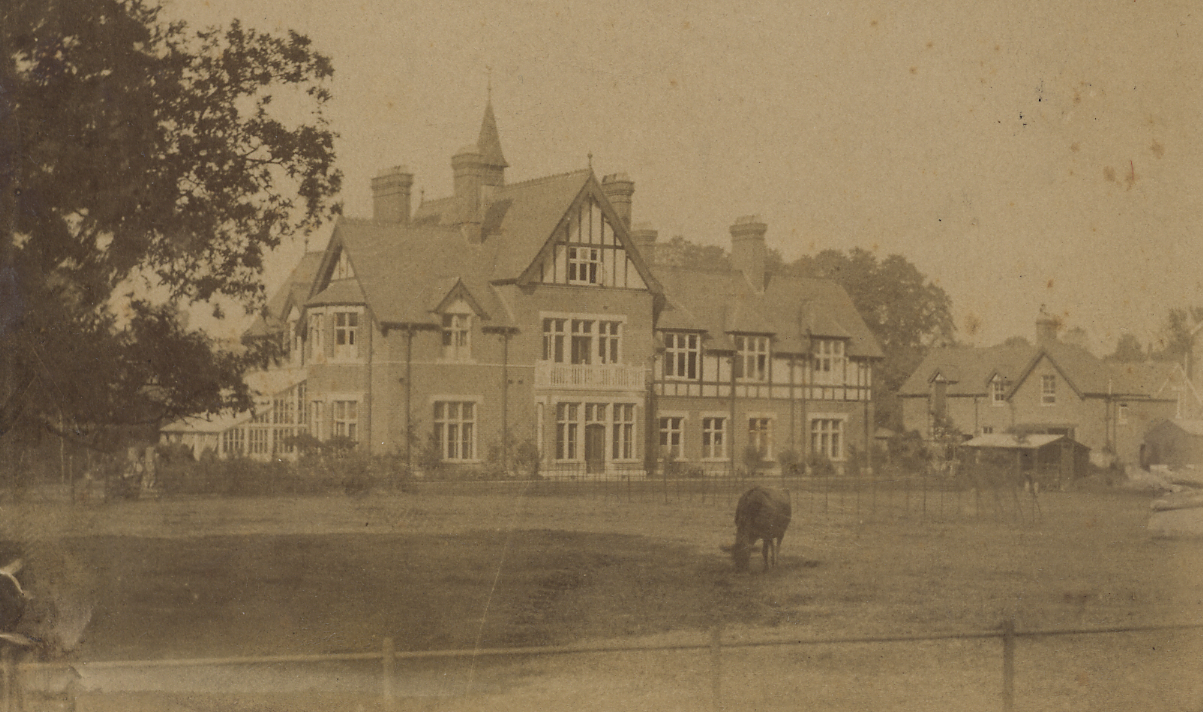
\includegraphics{photos/Mendips.png}
 \caption{The Mendips.}
\end{figure}

His obituary in the journal of the Rational Press Association reads:

\begin{quotation}
Obituary
DIED,
On January 15, 1918,
JOHN HILL MUNDAY,

A Director of the Rationalist Press Association, Limited, for over fifteen years.

Aged 73.

The death of Mr. J. H. Munday is a grevous loss to the Rationalist Press Association, of which he had been a Director since 1902, as well as its principal legal adviser. As senior partner in the firm of Messrs. Ellis, Munday, and Clarke, he was always busily employed, but he never failed to find opportunity to serve the R.P.A. in any capacity; and he rarely missed attending the Board meetings, where his shrewd and common-sense judgement was always invaluable to his colleagues. His kind and genial disposition won him a host of friends, while his unimpeachable integrity invited a confidence and trust which he regarded as one of his richest possessions. In his home circle he was an ideal husband and a devoted father, and it can truly be said of him that he was beloved by all who knew him.

[Transcription incomplete...]
\end{quotation}

The following funeral oration was given by Frederick Gould:\cite{JohnHillMundayFuneral}
 
\begin{quotation}
'Our dear friend, John Hill Munday, had, many years ago, courageously and decisively made up his mind as to his relations with his fellow-man and with nature at large. Towards his fellow-men his attitude was that of duty and honour. Towards nature his attitude was one of study and reasoned obedience, without any attempt to penetrate to supernatural secrets, or to spend golden time in discovering a world beyond death. In other words, he was both a good citizen and a staunch Rationalist. Such was his record, honest and clear, when he died at the age of 73. His memory is honoured by wife, son and daughters, and by his comrades in the struggle - the victorious struggle - for liberty and progress of thought. When, nearly twenty years ago, a small band of us laid the foundations of the Rationalist Press Association, our friend not only gave his sympathy to this effort on behalf of intellectual light for England and the world; he rendered substantial aid in drawing up the Articles of the new Association. For it was important, besides taking up the enterprise for freedom of the mind with enthusiasm, and to refine and state its objects with plainness, with precision, with business-like and prudent word and phrase so as to give confidence to supporters as well as candid and unmistakeable notice to the public. Trained and accustomed to the practice of law, our friend proved that he was both a good solicitor and and earnest disciple of Reason and Humanism. He took a seat willingly at the Board of the Association, and his fellow Directors found him, from the beginning and all the time, a most useful and competent colleague; not fond of much speaking, but attending with regularity and devoting careful consideration to all plans and proposals. Seven years ago, his keen legal eye detected certain points in the R.P.A. articles that needed improvement and safe-guarding. Like a man who schemes a building, and desires to lay its stones and beams truly and well, he framed a new statement, met his colleagues in many consultations, presided, discussed, persuaded, persevered, and so at length satisfied himself and his friends that the Association was solidly established and its aims more efficiently promoted. The work of months was tedious, but all was done with good heart and a valiant purpose. In matters of political and other opinions, he was for his own part firm and consistent; but towards those who differed, even towards the odd and eccentric, he was good-naturedly tolerant. It was therefor most natural that his colleagues should feel a very kindly attachment for him. On his retirement from partnership in his law-firm the R.P.A. Board assured him of their cordial respect. His reply intimated that, in co-operating for the spread of Rationalism (and hence for the welfare of mankind) he had spent the happiest hours of his life. It was, indeed, that fruitful kind of happiness which was good for the man himself, and good for world-wide humanity. And here may be noted two things in our friends' field of interest. He was always glad to hear of the extended circulation of books that aimed at the moral training of the young on humanist and rational lines. And he was specially active in the dispatch of our literature to soldiers engaged in the war, in camp or at the front; and may have been the evidences that such gifts were appreciated.

On the hearts of his wife and children is graven the recollection of his constant and tender thoughtfulness in the relationships and experiences of the home. Whatever may have been his sense of physical failure in the latter days, his master motive was to arrange affairs, to guard against discomforts, to provide for the future - in a word, to do all that a kind ingenuity and practical sense could suggest to ensure the peace and solace of those he loved, and assistance to the public cause for which he had so untiringly laboured. A man of absolute integrity in his business, a very loyal friend, a sure keeper of the plighted word, he was of simple taste and habit; and he desired this simplicity to mark the last rites. Hence we see here no crowding of memorial flowers. But there is at least one flower that we offer, and one that he would have thought of with a smile of gratitude - the flower of respect and hommage for a life of usefulness , of steady and brave conviction, of fidelity to an unpopular cause, of domestic affection and of generosity towards his fellow men."

Frederick J. Gould \\
Saturday 19th February 1918
\end{quotation}

The probate notice read: ``MUNDAY John Hill of Cedar Lodge 21 St Johns Road, Putney Hill, Surrey died 15 January 1918 at or near St Thomas Hospital Surrey. Probate London 12 March to the Public Trustee. Effects \pounds18,041.19s.1d (Will registered 1 December 1916).\cite{NationalProbateCalendar}

\biohead{Catherine Aldridge}{}


\biohead{Samuel Maxwell West Croskery}{Taken in Yokohama, Japan in 1905 and sent to his daughters.\cite{SMWCYokohama1905}}

West Croskery was born in 1847.\cite{SMWC-MG-marriage}

He married Mary Gilmour on 13 August 1874 in Troon (Ayrshire), when he was living in D\`{u}n Laoghaire, County Dublin, Ireland.\cite{SMWC-MG-marriage} They had two daughters: Nora (\p{Jeanie_Elenora_Dunsmuir_Croskery}) and Marian (\p{Marian_Gilmour_Croskery}).

Samuel became a Second Mate in Liverpool on 20 September 1869. There is an extensive record of all his subsequent voyages but some of this is unreadable.\cite{MarineRecordsSMWC} From 1869 onwards, he sailed to Australia, New York, Delaware, Nova Scotia, Singapore, Napier and Wellington (NZ), San Francisco, and Calcutta.

While Master of the Minterne (owner A.J. Hood) a typical short voyage was as follows: the ship left Antwerp on 5 December 1910, went to Huelva, Algiers, Genoa and Soulia. At that point he was 61 and signed himself as S.M. West Croskery, but the following year he signed as West Croskery. On this same voyage Clara Croskery (50) was listed as stewardess and paid One Shilling - her address was the same as Samuel's.

(The Minterne was struck and sunk by a German U-boat submarine in 1915.(Note 1) The crew were rescued and taken to Penzance and the newspapers wrote that he was the Captain at the time. However, Lloyds show his appointment as Master as being terminated in 1913, and there is no record on the ship's log of him at the time of the sinking.)

The following was published on the front page of \emph{The Morning Call} in San Francisco on 23 February 1895:

\begin{quotation}
\textsc{Blown to Sea in a Blizzard.}

\emph{Terrible Experience of the British Ship Benlarig.}

Baltimore, Feb. 22.---The steamer Rossmore arrived to-day with Pilot Franklin Beebe of New York and news of the overdue ship Benlarig, which left Caleta Buena, Chile, October 6, with a cargo of niter for New York.

She was seventy-five miles off New York February 5, when she took Pilot Beebe aboard to guide her into New York. Two days afterward the blizzard carried her to sea. All her sails were blown away. One of the crew was thrown and had a leg broken, and the intense cold prostrated three more with frost-bitten limbs. Two seamen died. The ship's company were put on short rations. After fourteen days' tossing about in the blizzard, the Rossmore, from Liverpool to Baltimore, sighted the ship on Monday night 130 miles off Sandy Hook. The Rossmore stopped and a boat put off from the distressed ship. Pilot Beebe was almost prostrated with illness. Captain Beall and seamen of the Benlarig refused to leave the ship. Captain Croskery supplied the ship's baot with food sufficient to last ten days. 
\end{quotation}

The following letter was written to his sister-in-law Mary Anne Mortimer Thomson:\cite{SMWCletter}
\begin{quotation}
\begin{flushright}
S. S. ``Rosmore'' \\
at sea \\
5\textsuperscript{th} June 1897
\end{flushright}

Dear Minnie,

I must tell you how shocked I was to hear of poor Alex's death. When I got home last voyage I had written you such a gossipy letter before, when at sea, I had let it go on, for I have such a short time in port that really I have not one minute to spare when in Liverpool. Last time only 54 hours so you see how quickly we are moved around.

Mary was very sorry. She always liked Alexander more than any of my brothers. He had such a kindly nature with him. Nora sent on your letter to Wallace at Eckington, and he sent word to Father. Poor old man he will I fear soon follow his Son. I have not seen him now for three years but hope to this fall. I fully expect that Mary and the two girls, Nora and Marion, will cross over to Dublin, when I return next to stay there for a month. I am sorry to say Mary is very far from well. Her heart has been giving her a lot of trouble as also a rupture of the navel, and being very stout, as you know, its very bad for her. However i hope the change, and at the sea shore, Bray or Dalthy, will do her good for she is a dear good wife to me, and I would not like to lose her. I am sure the old man will also be very pleased to see them again. I am sorry to say Fred's children do not pay the attention to Grandpa they ought do do, and so close to one another. Last voyage, I picked up 26 passengers of a shipwrecked steamer on the coast of Newfoundland, and brought them on to Liverpool. There was a very nice letter from them in the Liverpool papers of which I may be able to send you a cutting. I do not know if you will have heard of Capt. Herron, Capt. Weaver's father in law. He died just the day before I got in and I was at his funeral. His wife died just a month before. She head sailed always with him, and all the children were born at sea.

I was glad to hear your boys are able to do a little for you, dear Minnie, for you are and always were a brave woman, I was going to say girl but those days are gone, and I'm getting quite bray and bald myself. I see you have struggled nobly, so far, and I hope you will be able to pull through. I will not forget you now and again with a little help.

Does John live far from you? I suppose his son is also quite a big man and at business. Its a long time since I have had a lone from him; Kindly remember me to him.

I am now on my way to Montreal again. We generally take about 28 days on the round trip, so that I'm every month at him, although only for a short time. During winter the St Lawrence is all frozen up, and then its to Baltimore. last voyage out I had a dreadful time among the ice fields and thought at one time I was going to lose my shop as it was so dangerous among it. At the first of the season there is always a lot about. Our people are building a lot of new boats, and I'm in hopes of getting soon back in my old trade to Baltimore for this is far too risky a trade to be in with Ice, fogs and a bad coast to make. And there are times in fact nearly every voyage while close to the coast, I have not the clothes off me for five or six days. Nanie (?) Hugh's daughter which was over on a visit sailed for Jamaica a few days before I got home. She had been for six weeks in Downpatrick. But with two babies, it can't have been much pleasure. Charlie Hugh and Henry are the only two not married now. I don't have any word of Wallace. So I suppose he is going to be an old bachelor.

Now dear Minnie, I will say good bye and will post this when I get out. Give my love to each of the boys and my niece. Tell her I wish she was nearer us to visit her cousins who grieve for her loss. God bless and comfort you. Mary desired me to give you her love and made me promise to write you going out.

With much love to yourself \\
I am your affect Brother \\
West 
\end{quotation}

Minterne: Type: Steamer; GRT 3,018 tons; built GB 1903 by Richardson, Duck and Co, Stockton. Sunk by U-Boat U 30 (Erich von Rosenberg-Grusczyski) on 3 May 1915, 50 miles SW of Wolf Rock, en route Cardiff-Buenos Aires, carrying coal. 2 casualties (death of two firemen). (from www.uboat.net/wwi/ships)

Lloyds Registers show him as being Master of the following ships:\cite{LloydsRegCroskery}
\begin{itemize}[nosep]
\item 1865-69 Napier (iron barque) London-New Zealand, London-San Francisco)
\item 1870-71 Whittington
\item 1871 Lady Russel
\item 1873 Bristolian (\#44103) South Americas
\item 1874 Red Gauntlet (\#48809) East Indies
\item 1875 Stentor (\#70946) China, Japan, Oriental Arch.
\item 1876-78 Dawn (\#69262) Mediterranean
\item 1878-79 Olga (\#60222) Sunk outside Sulina 1 April 1879, raised 27 May 1879.
\item 1879-82 Bessarabin (\#78733) France, Portugal, Spain, Azores, Meditarranean,
\item United States, East Indies. Collison 21 February 1880.
\item 1883 Wallachia (\#87830) Mediterranean
\item 1884-85 Bessarabin "
\item 1885-93 Wallachia Mediterranean, United States, West Indies, Gulf of Mexico, Baltic States
\item 1893 Baltimore (\#91142) United States
\item 1894-97 Rossmore (\#96336) United States, British North America, Greenland, Iceland. Collision 30 August 1895.
\item 1898-99 Tropea (\#99433) United States
\item 1901 Birdoswald (was Tropea) "
\item 1901-03 Bedouin (\#105332) East Indies
\item 1905 Inkula (\#109335) China, Japan, Oriental Arch.
\item 1908-13 Minterne (\#118349) Australia, United States, India, Burma, Mauritius
\item 1913 Upcerne (\#120694) South America. Damaged by collision 29 October 1913, "colliding vessel alone to blame".
\end{itemize}

Appointment ceased 12 November 1913. (He was aged 63 at the time)

After he retired he lived at 9 Easton Road in New Ferry.
Died on 26 May 1933.\cite{WestCroskeryProbate}

Probate:\cite{WestCroskeryProbate}
\begin{quotation}
CROSKERY Samuel Maxwell West of 9 Easton-road New Ferry Cheshire died 26 May 1933 Probate Liverpool 11 July to Richard James Hancox bank inspector and Willian Davies Hughes estate agent.  Effects \pounds 8616 0s. 10d. Resword \pounds 8447 4s. 10d.
\end{quotation}

\biohead{Mary Gilmour}{c.~1890\cite{MaryGilmour1980}}

In the 1861 Census, Mary is 18 years old, living in Old Hurlford with her father Boyd (age 46), sister Marian (age 14), and brothers Boyd (age 12) and Allan Columbia (age 9). Her mother, Jean, had died in 1856.

When she marries Samuel Croskery on 13 August 1874, she gives her age as 29,\cite{SMWC-MG-marriage} but in fact she was 31 as she was born in 1843. 

\biohead{Harry Hancox}{}

\biohead{Maria Mary Merrett}{}

Maria Mary Merrett was born in Stroud, Gloucestershire in (about) 1845 to James Merrett (\p{James_Merrett}) and Elizabeth (surname unknown, \p{Elizabeth}).
She had  six siblings: William Merrett (c.~1842--?), Elizabeth Sarah Merrett (c.~1843--?), Catherine M. Merrett (c.~1848--?), Lucy Merrett (1852--1926), Richard H. Merrett (c.~1853--?), and Charlotte Merrett (c.~1857--?).

She married Harry Hancox (\p{Harry_Hancox}) on 28 May 1867 at St Stephen the Martyr, West Derby, Lancashire \cite{MariaMerrettMarriage}. They had four sons (see \p{Harry_Hancox}).

In the 1891 Census, Maria Mary was a widow and living at 30 Edge Lane. Her occupation was given as "Living on her own means" and she had her four sons at home: Harry was 22 (Bankers clerk), Frank was 21 (student of medicine), Charles was 19 (merchants clerk) and Richard was 17 (bankers junior clerk) \cite{MariaMerrettOccupation})

In 1901, she was 55, and had three of her four sons still living at home: Harry was 32 (a bankers clerk), Charles was 29 (office manager) and Richard was 29 (a bankers clerk); their address was 30 Edge Lane, Liverpool \cite{MariaMerrettResidence}.

She died on 22 October 1908 and was buried at Toxteth Park Cemetery on 24 October. \cite{MariaMerrettDeath}


% Generation 4
\biohead{Charles Frederick Barker}{c. 1850.\cite{CFBportrait}}

Charles Frederick Barker was probably born on 2 April 1801 in	Copenhagen, Denmark, although there is no primary record of this (as of January 2015).

The story handed down through the family is that he was born prematurely as a result of the bombardment of the city by Nelson on 1 April 1801. He was the son of the officer in charge of the Royal Armoury (Royal Armourer) in the Royal Danish Army, and was named after Charles Frederick, Prince of Hesse, brother of the Queen and Commander in Chief of the royal Danish Forces. He was a student at the Danish Military Academy, where it is said he could not tolerate the strict regime. (One of his contemporaries was Von Moltke, who joined the Prussian military school.) He ran away to sea at the age of 14 and landed in Whitby where he adopted the family name of Barker. (It is worth noting that on his Master's Certificate of Service (No.50,682), he has recorded his place of birth as Yarmouth, Norfolk and the date as 1 April 1800, although there is no record of his birth in the Norfolk records.) The information about his early life is taken from notes made by his son Thomas Henry Barker (held by living family member). According to these notes, he did go back to Copenhagen once, in 1850-1, to look for his sister (her name is not known).

He became a ship's apprentice in 1812 \cite{CFBShipList} and eventually became a master mariner (see below).

\begin{figure}
	\centering
	\begin{subfigure}{.48\textwidth}
		\label{Charles_Frederick_Barker_and_Elizabeth_Hezelwood}
		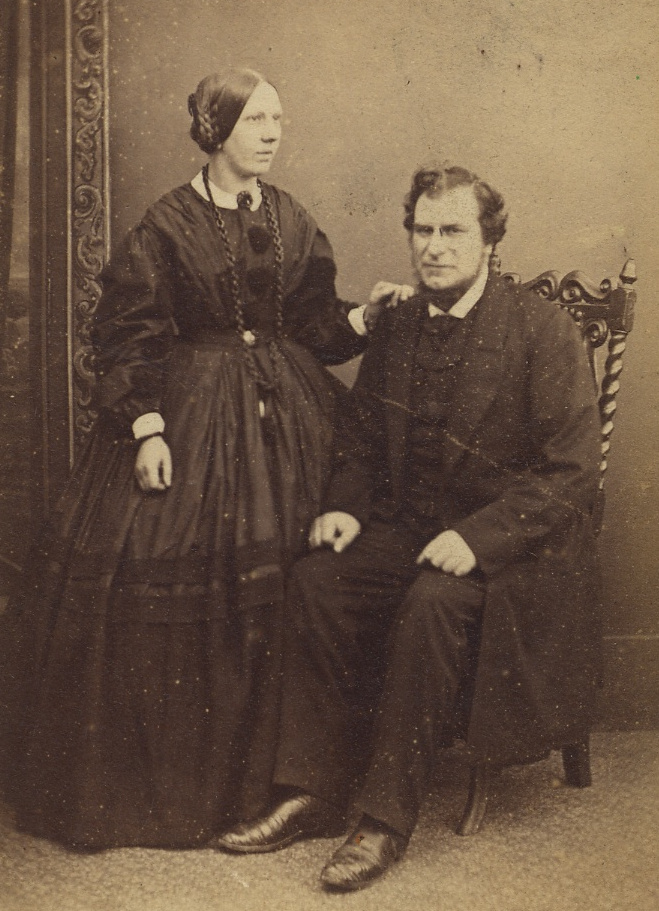
\includegraphics{photos/Charles_Frederick_Barker_and_Elizabeth_Hezelwood}
		\caption{Charles Frederick Barker and Elizabeth Barker (n\'{e}e Hezelwood, \p{Elizabeth_Hazelwood}).}
	\end{subfigure}
	\begin{subfigure}{.48\textwidth}
		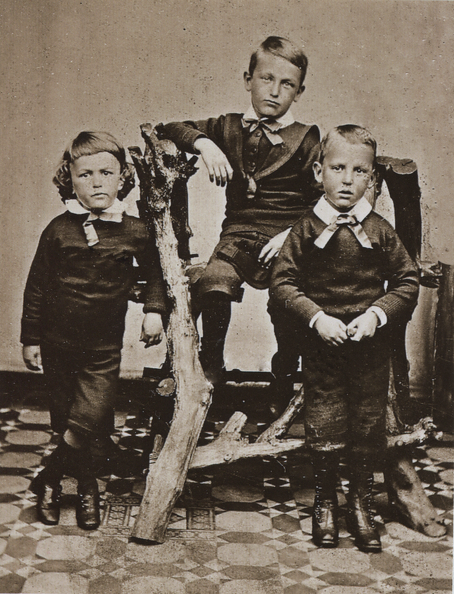
\includegraphics{photos/CFB_children.png}
		\caption{Charles Frederick Barker's children: Thomas Henry (\p{Thomas_Henry_Barker}), Charles Frederick, and Joseph Bolton.}
	\end{subfigure}
\end{figure}

He married Elizabeth Hazelwood (\p{Elizabeth_Hezelwood}) (whose name was originally spelt Hezelwood) of Whitby on 3 February 1836 at St. Dunstans, Stepney, Middlesex, and they lived in Stepney, Middlesex before later moving to Liverpool. They had four children: Charles Frederick Barker (1836--1887), who also became a mariner, Elizabeth Barker (1838--died in infancy), Thomas Henry Barker (\p{Thomas_Henry_Barker}) and Joseph Bolton Barker (1844--?). 

In 1851 the family was living at 8 Bickley Terrace, Toxteth Park, Liverpool and he was recorded as:
Charles Barker, Head. Ship master, aged 50, born Norfolk, Yarmouth. \cite{CFB1851}

His Certificate of Service in 1851 records his occupation as having been Chief Mate and Master for 39 years in the British Merchant Service in the Coastal and Foreign Trades. The ships that he served on, and in which capacity,  are shown as follows:

'Luna' (100 tons, Great Yarmouth) as Apprentice (Coal Trade), 1812 to 1817
'Lusitania' (300 tons, London) as Seaman (Cape and St Helena), 1818 to 1821
'Ellen' (300 tons, London) as Chief Mate (Mauritius), 1821 to 1827
'Morning Star' (245 tons,London) as Master (India), 1827 to 1830
'Hooghly' (500 tons,London) as Chief Mate (India), 1831 to 1833
'Bencoolen' (500 tons, London) as Chief Mate (India),1833 to 1835
'Euphrates' (600 tons, London) as Chief Mate (India), 1835 to 1837
'John Denniston' (500 tons,Greenock) as Master (India and South America) 1837 to 1840
'Ayrshire' (874 tons, Greenock) as Master (India) 1840 to 1844
'Baboo' (420 tons, Greenock) as Master (India and Australia) 1844 to 1850
'Ranee' (640 tons, Liverpool) as Master (India) 1850 to 1851
\cite{CFBShipList}


A hand written testimonial to Charles Frederick in recognition of his services to a passenger is held by a family member, and says:
"To Charles Barker, Esq., Commander of the Boboo,
From the Rev. J.Irvine, Vicar of Leigh.
In grateful acknowledgement of his courtesy, kindness and hospitality.
Plymouth Sound, 24 September 1848."

Later in the same year, the Baboo is listed as arriving in Adelaide, South Australia, from London and Plymouth, with Charles as Master, and a large complement of emigrants.\cite{CFBBaboo}

In 1853 he was sailing back to Liverpool, coming from Calcutta, via Rangoon and Mauritius ("Calcutta November 28th Ranee, Barker cleared for Rangoon Mussurel Munjeet, Fairweather, Mauritius" \cite{CFBRanee}) when he died at sea off the Cape of Good Hope on 14 July 1853 (the cause of death was unknown: however, there are many instances of mariners dying from yellow fever en route to Britain from India, noted in Liverpool newspapers of the period). It is recorded as  "Ships Spoke With: The Renee, Captain Barker (who died off the Cape), from Calcutta from Liverpool, July 24, in lat. 29 S, long. 11 E."\cite{CFBDeath}
He was buried at sea on the same day, off St. Simon's Bay. His eldest son, Charles Frederick Barker, was an apprentice seaman on the ship at the time - it was his first voyage at sea.

(His grandson and great grandson also served as RN officers. His grandson was the Commander of the Ardent and he was killed when she was sunk by the Germans in 1940. His great grandson was Nicholas Barker, Captain of the Endurance, who played an important role in the Falkland War.)


\biohead{Elizabeth Barker (n\'{e}e Hazelwood)}{}

Elizabeth was born on 5 April 1807 \cite{ElizabethHazelwoodBirth} in Whitby, Yorkshire, to  Moses Hezelwood (\p{Moses_Hazelwood}) and Elizabeth Mead (\p{Elizabeth_Mead}).  She had seven siblings: Mary Hazelwood (1805--1887), Isabella Hazelwood (1808--1882), Sarah Hazelwood (1811--?), Francis Mead Hazelwood (1813--?), Thomas Hezelwood (1814--1851), Francis Hazelwood (1816--?) and Trufit Mead Hazelwood (1817--?). 

She married Charles Frederick Barker (\p{Charles_Frederick_Barker}) on 3 February 1836 at St Dunstan's, in Stepney, Middlesex \cite{ElizabethHazelwoodMarriage} (although according to her brother Thomas in his notebook, held by a family member, they had left Whitby together to live in Stepney in 1834: ``My sister and Barker left Whitby on September 23\textsuperscript{rd} 1834.'')  They had three sons (one daughter died in infancy):  Charles Frederick Barker (1836--1887), Thomas Henry Barker (\p{Thomas_Henry_Barker}) and Joseph Bolton Barker (1844--?).

On 18 May 1841 they were living at 9 Earle Street, Liverpool \cite{ElizabethHazelwoodResidence}, and by 1851 they were in Toxteth Park, Liverpool, Lancashire. In July 1875 she had moved to	Peckham, Surrey,15 Ryder Villas, St Mary's Road, Peckham, Surrey to live with her youngest son, Joseph: letters from Elizabeth (held by family member) in 1875 to her daughter-in-law (married to Thomas Henry, known as Tom) show that she was living with her son Joseph (Joe) and she welcomes Mary into the family. She also enquires into the health of Mrs. Denton (Mary's aunt). In 1878 she writes about her sister Maria, who is living with Tom and Mary. In 1881, Elizabeth had moved to live (with her son Joe) in Streatham. 

Shortly before her death she wrote the following letter with regard to her private property: (On an envelope addressed by Mrs Barker, 2 Ryden Villas, Rossiter Rd, Balham):

\begin{quotation}
My dear children Charles Tom and Joe I have for a long time thought of putting down on paper my wishes with regard to the few things I posess (sic) . There is not much of value only for the sake of them having belonged to your dear Father and Mother. I cannot make an equal distribution as Joe’s house has so long been my home that I consider he ought to have xxx in the first place. I should (line through) wish him to have the things in my bedroom, that is bedstead bed bedding drawers washstand dressing table chairs \& carpet and glass --- there are a few things of your dear Fathers bringing I should like you each to have one of the two large vases china dish and stand and the bamboo ornaments and small vases --- beside many little things. I cannot name my books I wish Charles to have Fletchers family devotion Tom Pilgrims progress Joe Sundays at home and divide according to your own judgement Tom gave me many of them and can choose for himself the one over the dining room mantle piece is the only one of value. Tom can have his oil paintings if he xxx Mr Birkett’s oil paintings xxxxxxx Tom always thought he had a right to them these things I must leave to your own judgment as(?) with regard to bed linen what I have is nearly worn if you would like to divide it My clothes whatever would be useful to my sister if she survives me I wish her to have The rest divide as you like and let it all be done peaceably my ?? only the brooches the larger with your dear Father’s hair. I wish Charles to have for Barbara the amythest. And the little pe... that was Mrs ,,,,,,,,,,, Tom to have for Mary, and a small black one Joe for Millie
My old watch for Ida and the little seal and key for Hilda my chain I should like cut in two and half for Harry and half for Jimmie when old enough they could dispose of it to go toward buying........"
\end{quotation}

Held in personal papers.

Elizabeth died on 17 December 1882 Liverpool, Lancashire at 134 Windsor Street, Liverpool and was buried on 24 December at the Anfield Cemetery, Liverpool. \cite{EHazelwoodDeath}

\biohead{John Moulsdale}{}

John Moulsdale was born before 1825.  He married \bioref{Maria_Jackson} in April 1844 at St. Nicholas Church, Liverpool, Lancashire \cite{JohnMoulsdaleMarriage}.
They had three daughters: \bioref{Mary_Ellen_Moulsdale}), Maria Moulsdale (1857--?), and Sarah Ann Moulsdale (1857--?).
His occupation in 1875 was as a Book-keeper \cite{JohnMoulsdaleOccupation}.

\biohead{Maria Jackson}{}
\index{Jackson, Maria}

Maria Jackson was born in 1815 to March (\p{March_Jackson}) and Ann (n\'{e}e Holmes, \p{Ann Holmes}) Jackson. She married John Moulsdale (\p{John_Moulsdale}) and died in 1863.

\biohead{William Munday}{}

William Munday was born on 7 August 1800 \cite{WillMundayBirth} in Bishopstrow, near Warminster, Wiltshire, to James Munday (\p{James_Munday}) and Jemima Browne (\p{Jemima_Browne}).  He had eight siblings:  Jemima Munday (1798-1870), Catherine Munday (1802-1883), Sarah Munday (1803-1869), James Munday (1805-1863), Mary Elizabeth Munday (1807-1896), John Munday (1809-1835), Henry Thomas Munday (1813-1895) and George Munday (1815-1830).

He married Mary Hill (\p{Mary_Hill}) on 1 December 1835 in Paulton, Somerset and they had ten children:  George Hill Munday (1836-1862), Captain James William Munday (1838-1875), Mary Elizabeth Munday (1840-1849), Anna Maria Munday (1841-1895), Sarah Adeline Munday (1843-1924), John Hill Munday (\p{John_Hill_Munday}), Thomas Hill Munday (1846-1862), Walter Edward Munday (1847-1932), Nelson Munday (1848-1886) and Louisa Fry Munday (1851-1881).

From 1837 until 1858 he was a wine merchant in Weymouth Street, Warminster, Wiltshire \cite{WillMundayOccupation}. William Cobbett wrote in 1826 in 'Rural Rides' that: "Warminster is a very nice town; everything belonging to it is solid and good."   Despite this, they later moved to Battersea, and lived at 32 Middleton Road,  where he was still a wine and spirit merchant until retiring in his late sixties \cite{WillMundayBattersea}.

He died on 26 December 1886 and was buried at Norbiton Cemetery, Surrey on 29 December \cite{WillMundayDeath}.




\biohead{Mary Hill}{Mary Hill}{}

Mary Hill was born in 1809, married John Hill Munday (\p{John_Hill_Munday}) on 1 December 1835, and died in 1879.

\biohead{Napoleon Aldridge}{}

Napoleon Aldridge was born on 25 October 1801 in Oxford, Oxfordshire to Edward Henry Aldridge (\p{Edward_Henry_Aldridge}) and Leah North (\p{Leah_North}) \cite{NapoleonAldridgeBirth} and was baptised on 16 April 1802 at St Mary the Virgin (University Church), Oxford by the Rev. E. Coplestone.  He had four siblings:  Judith Aldridge (1794-?), Virginia Aldridge (1796-?), Leah North Aldridge (1798-?), and Edward Henry Aldridge.

He married Mary Ann Chymist (\p{Mary_Ann_Chymist})on 1 April 1832 at St Giles in the Fields, Camden, London \cite{NapoleonAldridgeMarriage}  (he is noted on the certificate as "widower"; however, there is no evident record of a previous marriage) and they had eight children:  Edward Henry Aldridge (1832-1899),  Napoleon Alfred Aldridge (1836-1905), Leah North Aldridge (1837-1912), Virginia Elizabeth Aldridge (1839-1912), William Aldridge (1843-?), Alice Judith Aldridge (1845-?), Alfred Frank Aldridge (1846-?) and Catherine Aldridge (\p{Catherine_Aldridge}).

In 1851 he was working as the Senior Clerk to the Master of the Queens court in London and they lived at 18 Crouch Hill Road, Islington, Middlesex \cite{NapoleonAldridgeOccupation}.  In 1861 the Census lists him as being the Chief Clerk of the Masters Office, Court of Queens Bench, and also as a farmer, living at Hill Farm, Green Lane, Sutton Common \cite{NapoleonAldridgeResidence}.  He was farming about 90 acres of land, employing 3 men and 2 boys.  Ten years later he had retired.
	
He died on 1 Aug 1875 at Oakfield House, Sutton, Surrey \cite{NapoleonAldridgeDeath}.


\biohead{Mary Ann Chymist}{}
\biohead{Hugh Croskery}{}

\begin{figure}
 \centering
 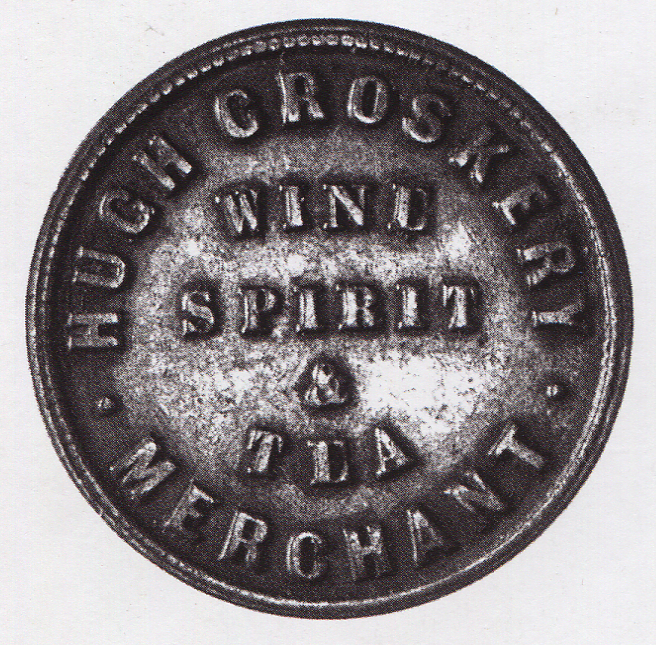
\includegraphics{photos/Hugh_Croskery_token}
 \caption{A `token' from Hugh Croskery's grocery shop.\cite{DownTown2}}
\end{figure}

Hugh Croskery was born in 1803, in Downpatrick, County Down, Northern Ireland (his parents are not known).

He married Charlotte Wallace Brown (\p{Charlotte_Wallace_Brown}) on 9 May 1834 at the First Presbyterian Church, in Ballynahinch, County Down and they had eight children:  Hugh Croskery (1835-1886), Ann Croskery (1836-1931), Alexander Brown Croskery (1838-1897), Albert James Croskery (1840-1865), Horatio Collingwood Croskery (1842-1929), Frederick C. Croskery (1845-?),  Captain Samuel Maxwell West Croskery (\p{Samuel_Maxwell_West_Croskery}) and Wallace Brown Croskery (1851-1926). 

His occupation was as a Grocer, wine, spirit and general merchant, in 1846 living in Scotch Street, Downpatrick and then in Market Street in 1850. An advertisement in the Downpatrick Recorder on 30 November 1847 read:
``Wanted: an Apprentice to the Spirit and Grocery Business. Apply to the Subscriber, Hugh Croskery.''\cite{HCroskeryAdvert}  He was also a publican in Scotch Street \cite{HughCroskeryOccupation}. By 1874 his occupation was noted as being a retired Ship owner, and he was also a mine owner and farmer. 

He died after 1897: at the time he was living in Dublin (as mentioned in a letter dated 1897 from his son West to his daughter-in-law Minnie, after his son Alexander had died in New Zealand (\p{Samuel_Maxwell_West_Croskery}). \cite{HughCroskeryDeath}.


\biohead{Charlotte Wallace Brown}{}

Charlotte Wallace Browne was born in or about 1813, in Ballynahinch, County Down, Northern Ireland \cite{CharlotteWBrowneBirth}, to Alexander Browne and an unknown mother.

She married Hugh Croskery on 9 May 1834 at the First Presbyterian Church in Ballynahinch and they had eight children (see page \pageref{Hugh_Croskery}).

She was still alive on 13 August 1874 as she was present at the wedding of her son Samuel Maxwell West Croskery to Mary Gilmour in Troon, Ayrshire, Scotland. \cite{SMWCmarriage}

\biohead{Boyd Gilmour}{Boyd_Gilmour}{}

Boyd Gilmour was born on March 22, 1814, in Riccarton ("Gilmour Riccarton 3 April 1814 this day was baptized Boyd son of Joseph Gilmour and Mary Clark born 22 Mar."\citeref{BGbirth}) and died on 26 March 1869 (Ayrshire, Scotland).  His parents were Joseph Gilmour (\p{Joseph_Gilmour}) and Mary Boyd Clark. His siblings were Elizabeth Gilmour (1797--1870), Joseph Gilmour (1802--1851),
James Gilmour (1805--1866), Allan Gilmour (1807--1854), Andrew Gilmour (1810--1874), Robert Gilmour (1812--1841).


He married Jean Dunsmore (Dunsmuir) and they had eight children:  Jean Gilmour (1836--?), Joseph Gilmour (1838 -- bef. 1840),\citeref{JGbirth} Joseph Gilmour (1840--?), Mary Gilmour (1843--1899),  Marion Gilmour (1847--1928), Boyd Gilmour (1849--?), Allan Columbia Gilmour (1851--?), John Gilmour (1854--1856).

After her death he remarried Elizabeth Howatson.

On 19 December 1850, Boyd and his family sailed on the Pekin for Fort Vancouver, and the journey took 191 days. On 18 July 1851 they sailed to Fort Rupert, on Vancouver Island where he took up a contract to develop new coal mines for the Hudson Bay Company (the HBC had recruited expert miners and their families on three-year contracts from the Orkney Islands and the county of Ayrshire). He struggled unsuccessfully to develop a producing coal operation, (with his nephew Robert Dunsmuir, who was to become one of the richest men on the west coast) at Fort Rupert. Life at Fort Rupert was harsh. When the miners arrived they found no working mine, inferior coal, food shortages, and danger from warring native tribes. The settlement consisted of a defensive wooden surround in the traditional wild-west style, and single room log cabins with a central stone fireplace and bunk beds set against the wall. Water was drawn from a communal well: communal ovens were used for cooking. The coal there was poor, so Fort Rupert’s mines were eventually abandoned after many miners breached their contracts and fled to the California gold fields. (S6) Those few that remained moved to Fort Victoria, including Boyd and his family, on 24 August 1852 after Governor Douglas instructed them to move 200 miles south to Nanaimo, a small port which was based on the fur trade and fishing. It was here that a local Indian told the settlers where they could find stones that burn - thus a coal seam was discovered. Work proceeded but living conditions were difficult. Living conditions were only slightly better at Nanaimo and Jean Gilmour refused to live there. The Gilmours returned to Scotland in 1854, when Governor Douglas refused to increase their pay rates.

After Jean died in 1856, Boyd is shown in the 1861 Census as living in Old Hurlford and is a Coalmaster (widower,age 46) with his children Mary (18, \p{Mary_Gilmour}), Marian (14), Boyd (12), and Allan Columbia (9). He then remarried later that year (11 November) to Elizabeth Howatson, a 20 year old farmer's daughter (living at Hill Farm) and had three more children.
When his daughter Mary married Samuel West Croskery in ? his occupation was noted as Coalmaster.\citeref{Marriagecert}

In the 1868 Hurlford District Directory his properties are listed as Woodend, Burnbank, Ladyton, and Goatfoot Collieries.

On his death certificate he is listed as "Coalmaster", and died at his home, "Riverside Cottage", Loudon Parish. His father Joseph was down as a coal miner. He died from 'fatty degeneration of the heart ten days from appearance of symptoms' and the death was reported by his brother Andrew Gilmour, butcher, also of Loudon Parish. His will includes details about a contract with his son Allan, and provision is made for his second wife Elizabeth (use of his house in Titchfield Street, Galston, and a yearly annuity of (pounds) 120 until the youngest child attains the age of 21 after which the entitlements were reduced - payable Whitsunday and Martinmas. Plus reasonable assistance after his death to provide his wife and children with mourning. When or if she remarries, she would then receive (pounds) 20 per annum. She "is obliged to maintain and upbring in a manner suitable to that station such of his children who have not attained majority.")(S6 

\begin{references}
 \reference{Marriagecert}{Marriage record of Samuel Croskery and Mary Gilmour}
\reference{BGbirth}{Birth record of Boyd Gilmour, Scotlands People, 03/04/1814 O.P.R.births 611/00 0010 0319}

\reference{JGbirth}{ Scotlands people, BIrth records, Riccarton Parish, record no.611, vol.0020}

%\reference{LABEL}{Citation text.}

\end{references}

\biohead{Jean Dunsmore}{}

Jean Dunsmore (also known as Jeanie Dunsmuir) was born on 8 December 1816 in Kilmarnock, Ayrshire, Scotland to Robert Dunsmore (\p{Robert_Dunsmore}) and Jean Kirkland (\p{Jean_Kirkland}).  She had four siblings:  James Dunsmuir (1805--1832), Marian Dunsmuir (1808--1872), Allan Dunsmuir (1847-?),  and Mary Dunsmore (1810, died in infancy).

She married Boyd Gilmour (\p{Boyd_Gilmour}) on 26 June 1835  in Riccarton, Ayrshire, Scotland \cite{JeanDunsmoreMarraige} and they had eight children:  Jean Gilmour (1836--?), Joseph Gilmour (1838-died in infancy), Joseph Gilmour (1840--?), Mary Gilmour (\p{Mary_Gilmour}), Marion Gilmour (1847--1928), Boyd Gilmour (1849--?), Allan Columbia Gilmour (1851--?) and John Gilmour (1854-1856).

She already had five children when they left on the Pekin on 19 December 1850 to sail to Vancouver Island where Boyd had been employed to open up coal mines in the north. Jean gave birth to Allan Columbia as the ship sailed up the Columbia river, and they arrived at Fort Vancouver on June 29 1851 (see \p{Boyd_Gilmour} for further details of their time in Canada).  

Jean died age 38 from "enteritis, 2 days"  on 16 May 1856 soon after her youngest son's death \cite{JeanDunsmuirDeath}, only two years after they returned from Canada, and she is buried in Riccarton Burial Ground.

\biohead{Thomas Elias Hancox}{}

Thomas Elias Hancox was born in 1806 in Shilton, Warwickshire \cite{TEHancoxBirth} to \bioref{Thomas_Hancox} and \bioref{Sarah_Jackson}.

He married \bioref{Frances_Heeley} on 2  May 1830 at St Philips Church, in Birmingham, Warwickshire and they had five children: Thomas Elias Hancox (1831--?), William Hancox (1833--?), \bioref{Harry_Hancox}, Frances Hancox (1838--1852) and Emma Hancox (1847--?).

In 1851, his occupation was given as a Webb and Clog maker, and they lived at 4 Duddeston Road, Birmingham \cite{TEHancoxOccupation}.

In 1867 he was living in Liverpool, Lancashire and is listed as being a "Gent" on his son Harry Hancox's marriage certificate \cite{TEHancox1867}.

He died in 1884 in Aston, Warwickshire (no citation available).

\biohead{Frances Heeley}{}

\biohead{James Merrett}{}

James Merrett\cite{HH-MMM-marriage} was born in 1813 in Wotton-under-Edge in Gloucestershire, England.
His father was \bioref{William_Merrett}, a dyer.\cite{MerrettCoppinMarriageCert}

On 6 April 1841 he married \bioref{Elizabeth_Coppin}.\cite{PeterKarpinski_2016-04-04,MerrettCoppinMarriageCert}
They had seven children: William Merrett (abt 1842--?), Elizabeth Sarah Merrett (abt 1843--?), \bioref{Maria_Mary_Merrett}, Catherine M. Merrett (abt 1848--?), Lucy Merrett (1852--1926), Richard H. Merrett (abt 1853--?), and Charlotte Merrett (abt 1857--?). 

By 1851 he was working as a dyer in Stroud;\cite{Census1851Merrett}; ten years later he was still in the same trade and had progressed to employing twenty-three men and a boy.\cite{Census1861Merrett}

He died on Christmas day in 1862 in Bowbridge in Stroud. Probate was announced as follows:\cite{JamesMerrettProbate}

\begin{quotation}
28 February 1863: The Will of James Merrett formerly of Gunhouse but late of Bowbridge both in the Parish of Stroud in the County of Gloucester Dyer deceased who died 25 December 1862 at Bowbridge aforesaid was proved at Gloucester by the oath of Elizabeth Merrett of Bowbridge aforesaid Widow the Relict the sole executrix. Effects under \pounds2000.
\end{quotation}

\biohead{Elizabeth}{}

Elizabeth (maiden name unknown) was born in about 1812 in Fairford, Gloucestershire, England.\cite{Census1861Merrett}

She married James Merrett (\p{James_Merrett}) and they had seven children (see\p{James_Merrett}).


\chapter{Data}
\input{census}

\begin{thebibliography}{99}

\bibitem{MaryGilmour1980}
	Mary Gilmour, c.~1890.
	\url{http://photos.samwilson.id.au/picture/1726}

\bibitem{FrankHeeleyHancoxResidenceUK}
	1891 Census: RG2/2990.

\bibitem{HarryMerrettHancoxDeath}
	England and Wales, National Probate Calendar (Index of Wills and Administrations), 1858--1966.

\bibitem{PhyllisWickhamDeath}
	England \& Wales, Death Index: 1916--2006. Vol.~10f; p.~1628.

\bibitem{THBcensus}
	283 MRG/3/1, in the Liverpool records office.

\bibitem{Census1871-3823}
	1871 Census. Class: RG10; Piece: 3823; Folio: 108; Page: 29; GSU roll: 841915.

\bibitem{JohnHillMunday1911}
	UK Census 1911; Rg 26, ED 13, Piece 244.

\bibitem{JohnHillMunday1881}
	1881 UK Census: Kingston, V. 26; Piece 837, Folio 87, p.36.

\bibitem{JohnHillMunday1871}
	1871 UK Census: Battersea EN 23; 133; Piece: 703, Folio 128, p. 35.

\bibitem{JohnHillMundayJudgement}
	Judgments---Prince Jefri Bolkiah v. K.P.M.G (A Firm), in \emph{House of Lords Judgements}, 18 December 1998.
	See \url{http://www.publications.parliament.uk/pa/ld199899/ldjudgmt/jd981218/prince02.htm}
	or alternate archive at \url{http://www.webcitation.org/6859rbdqW}

\bibitem{HeaddingtonMannor}
	\emph{The Manor of Heddington}, in Headington, Oxford, 2012-06-01.
	See \url{http://www.headington.org.uk/history/heddington_manor/index.htm} or alternate archive at \url{http://www.webcitation.org/6859cNV6m}

\bibitem{EGWHchristening}
	England \& Wales Christening Records, 1530--1906.
	Place: Rock Ferry, Cheshire, England; Collection: St Peter; Date Range: 1871--1919; Film Number: 1656759.

\bibitem{ToxtethParkCemeteryInscriptions}
	Toxteth Park Cemetery Inscriptions, M 25 BARKER. (C.Q.163). \url{http://toxtethparkcemeteryinscriptions.co.uk}

\bibitem{ToxtethBarker20}
	Toxteth Park Cemetery Inscriptions. P 20 BARKER. (C.Q.50).
	Large flat rectangular sand-stone, missing top/central cross? Inscription:
	``In loving memory of / Thomas Henry BARKER, / who departed this life April 9th 1917, / aged 75. /
	Also of Mary Ellen, / wife of the above T H BARKER, / died December 14th 1936, / aged 91.''
	\url{http://www.toxtethparkcemeteryinscriptions.co.uk/?search-class=DB_CustomSearch_Widget-db_customsearch_widget&widget_number=preset-default&cs-post_title-0=barker&cs-all-1=1917&cs-all-2=&cs-all-3=&search=Search}

\bibitem{WestCroskeryProbate}
	\emph{Index of Wills and Administrations record for Samuel Maxwell West Croskery},
	National Probate Calendar for England and Wales 1861--1941.

\bibitem{UKCensus1911_RG14_22074}
	1911 Census of England. Class: RG14; Piece: 22074.

\bibitem{UKCensusRG11_3688}
	UK National Archives. Public Record Office (PRO) RG 11 General Register Office: 1881 Census Schedules.
	Class: RG11; Piece: 3688; Folio: 55; Page: 37; GSU roll 1341883.

\bibitem{VirginiaDocs}
	\emph{Personal documents of Virginia Gregenik}, held by Peter Grebenik.

\bibitem{FlickrMarianGilmourCroskery}
	Portrait of Marian Gilmour Croskery, c. 1904.
	\url{https://www.flickr.com/photos/freosam/15608155092/}

\bibitem{FlickrJohnHillTree}
	John Hill's family tree \url{https://flic.kr/p/nszZrK}

\bibitem{JHM-CA-marriage-announcement}
	\emph{The Times}, Sat. 10 April 1880. 

\bibitem{JHM-CA-marriage}
	Marriage certificate of John Hill Munday and Catherine Aldridge
	\url{http://photos.samwilson.id.au/picture/1559/category/175}

\bibitem{JDB_BirthCert}
	Birth Certificate of James Denton Barker, August 1876. General Register Office.
	\url{https://www.flickr.com/photos/freosam/15452735948}
	Accessed: 27 October 2014.

\bibitem{SMWCmarriage}
	\emph{Marriage record of Samuel Croskery and Mary Gilmour}, August 1874.
	Statutory Marriages 590/02 0013. Scotland's People,
	\url{https://archive.org/details/MarriageRecordOfSamuelCroskeryAndMaryGilmour}
	Accessed: 8 November 2014.

\bibitem{BGbirth}
	Birth record of Boyd Gilmour,
	Scotland's People 03/04/1814 O.P.R.births 611/00 0010 0319,
	Transcript: ``Gilmour Riccarton 3 April 1814 this day was baptized Boyd son of Joseph Gilmour and Mary Clark born 22 Mar.''
	\url{https://archive.org/details/RecordOfBirthOfBoydGilmourEtAl} accessed 9 November 2014.

\bibitem{JGbirth}
	Riccarton Parish birth records, record no. 611, vol. 20. Scotland's People.

\bibitem{BGobituary}
	\emph{Obituary}, Kilmarnock Standard (newspaper), 3 April 1869. Burns Archives, Kilmarnock.

\bibitem{USCities}
	U.S. City Directories, 1821-1989.

\bibitem{NYpassengers}
	New York Passenger Lists, 1820--1957. Year: 1934; Microfilm Serial: T715; Microfilm Roll: T715\_5545; Line 5, p.\ 33.

\bibitem{EGWHbirth}
	FreeBMD, Wirral Births Sep 1911. Vol.\ 8a, p.\ 824.
	\url{http://www.freebmd.org.uk/cgi/information.pl?cite=LJ2MWUqdWRLxmn899\%2B7Fog&scan=1}


\bibitem{USCanadaBorderCrossings}
	Border Crossings: From Canada to U.S., 1895-1956.
	National Archives and Records Administration (NARA), Washington, D.C.
	Manifests of Alien and Citizen Arrivals at Babb, Montana, June 1928 -- October, 1956.
	Record Group: 85, Records of the Immigration and Naturalization Service; Microfilm Serial: A3386; Microfilm Roll: 1.

\bibitem{BMDIndex_RalphMundayDentonBarker_birth}
	General Register Office Index to Births, Marriages, and Deaths.
	Births Sep 1916, Birkenhead district, p. 927, vol. 8A.
	\url{http://www.freebmd.org.uk/cgi/information.pl?cite=4\%2BtKOMx5ci07jzFY0DkU9Q&scan=1}

\bibitem{FlickrRalph}
	Group photo of teachers at Ralph's school, c.\ 1935.
	\url{https://www.flickr.com/photos/freosam/13988198711}

\bibitem{MarriageCertRalphDentonBarkerJoanNyriaPowell}
	General Register Office, 1947. Certificate of marriage of Ralph Denton-Barker and Joan Nyria Powell.
	Details: Ralph Munday Denton Barker: aged 30, bachelor; Profession: School Master;
	residence at time of marriage: 2 Rookfield Close N10; father: James Denton Barker, Averadge Adjuster (retired).
	Joan Nyria Powell formerly Hancox: aged 29, the divorced wife of Geoffrey George Powell;
	residence at time of marriage: 2 Rookfield Close N10; father: Richard James Hancox, Bank Manager (retired).
	Marriage witnessed by E. M. Mitchell and K. Barker.
	\url{https://archive.org/details/CertificateOfMarriageOfRalphMundayDentonBarkerAndJoanNyriaHancox}

\bibitem{EGWMbirth}
	England \& Wales, FreeBMD Birth Index, 1837--1915.

\bibitem{1881censusKingston}
	1881 England Census. Reg. Kingston, v.26, Piece 837, folio 87, p.36.

\bibitem{1891census}
	1891 England Census. Kingston, V.22; Piece 612, Folio 67, p.34.

\bibitem{EGWHborder}
	Border Crossings: From Canada to U.S., 1895-1956.
	National Archives and Records Administration (NARA); Washington, D.C.; Manifests of Alien and Citizen Arrivals at Babb, Montana, June 1928-October, 1956; Record Group: 85, Records of the Immigration and Naturalization Service; Microfilm Serial: A3386; Microfilm Roll: 1.

\bibitem{CasaP1}
	\emph{Recognition Given U Of A By British}
	Casa Grande Dispatch (Tucson, Arizona, USA), p. 1 25 May 1934. \url{http://www.newspapers.com/newspage/13955618/}

\bibitem{BMDIndex_JoanNyriaHancox_birth}
	GRO index to Births, Deaths, and Marriages,
	Bebington district. Record name: Joan M [sic] Hancox.
	1918 p. 582 vol. 8A.

\bibitem{1901censusMendips}
	1901 England Census. Kingston v.356; Piece 667, folio 63, p.63

\bibitem{NyriaBirth}
	Birth Certificate. General Register Office.
	1918. Birth in the sub-district of Bebington in the County of Chester.
	Registration number 282, 4 March 1918.
	\url{https://archive.org/details/CertificateOfBirthOfJoanNyriaHancox}

\bibitem{NyriaChristening}
	England \& Wales Christening Records, 1530-1906.
	Place: Rock Ferry, Cheshire, England; Collection: St Peter;
	Date Range: 1871--1919; Film Number: 1656759.

\bibitem{FlickrNyria}
	Photograph of Nyria in Great Witley in the late 1950s,
	\url{https://flic.kr/p/njVZw3}.

\bibitem{OralHistoryJDB2008}
	Oral history interview with Julia Denton-Barker, 2008.

\bibitem{THBbio}
	\emph{Biography of Thomas Henry Barker}, author unknown, c.\ 1920.
	\url{https://en.wikisource.org/wiki/Biography_of_Thomas_Henry_Barker}

\bibitem{Echo1917}
	\emph{Liverpool Echo} newspaper, 10 April 1917.

\bibitem{THBfreebmd}
	FreeBMD record, retrieved 31 August 2014. GRO entry: Wirral 8a/504.
	\url{http://freebmd.org.uk/cgi/information.pl?r=137462560&d=bmd_1407157232}
	\emph{Deaths June 1917: Barker, Thomas H. (age 75)}

\bibitem{THBbirth}
	General Registry Office, birth certificate BXCF518186.

\bibitem{THBresidence}
	Class: RG12 Piece 2976; folio: 15; Page 26; GSU roll: 6098086.

\bibitem{THBplantagenets}
	\emph{Descent of Thomas Henry Barker from the Plantagenets},
	handwritten document.

\bibitem{THBmarriage}
	Marriage certificate of Thomas Henry Barker and Mary Ellen Moulsdale, 25 August 1875.
	\url{https://www.flickr.com/photos/freosam/15441758029/}

\bibitem{RalphMundayBMD}
	 Western Australian Registry of Births, Deaths and Marriages, Perth district registration number 3064.
	 Entry: ``MUNDAY RALPH 	Male 	77 	JOHN H 	CATHERINE 		PERTH 	3064 	1962''.

\bibitem{Aquariums}
    Cottesloe Aquarium Is Fish Fairyland.
    (1949, October 2). Sunday Times, p. 12. Retrieved November 6, 2014,
    from \url{http://nla.gov.au/nla.news-article59495916}.

\bibitem{LadiesSection}
	The LADIES' SECTION. (1926, August 22). Sunday Times, p. 1 Section: Fourth Section.
	Retrieved November 6, 2014, from \url{http://nla.gov.au/nla.news-article58247537}.
	``Miss Vera Maunder, of Cottesloe, left last Sunday by the Gascoyne for Java, where her marriage to Mr. Ralph Munday, formerly of Cottesloe, will take place; Prior to her departure Miss Maunder was presented with a handsome travelling case by the members of the Cottesloe District Tennis Club at their last monthly dance.''

\bibitem{VMkal}
	A LADY'S LETTER. (1923, April 27). Kalgoorlie Miner, p. 3.
	Retrieved November 6, 2014, from \url{http://nla.gov.au/nla.news-article87321886}
	``Miss Vera Maunder, of the Education Department, took her departure for Perth by Tuesday's train.
	Miss Maunder has been transferred to the West Leederville State School.''

\bibitem{BMD1907}
	FreeBMD, Birkenhead Births Dec 1907 8a/549.
	\url{http://www.freebmd.org.uk/cgi/information.pl?cite=7z1yGRD35cfIhArn\%2Bmzhzg&scan=1}, Accessed: 27 October 2014.

\bibitem{1911Census}
	1911 UK Census.

\bibitem{1911censusWandsworth}
	1911 Census. Wandsworth; Reg.26; ED.13, Piece 2444

\bibitem{FreeBMD-CA}
	Birkenhead, in England \& Wales, FreeBMD Death Index, 1837-1915, Vol. 8a p.617, June 1922.
	\url{http://www2.freebmd.org.uk/cgi/information.pl?r=147285680&d=bmd_1373527565}

\bibitem{SMWC-MG-marriage}
	Marriage record of Samuel Croskery and Mary Gilmour
	\url{http://photos.samwilson.id.au/picture/1725}

\bibitem{MarineRecordsSMWC}
	National Archives, Kew, London.
	Marine records: BT115/3, BT/122/62 (1869-1888), BT122/85 (1885-1894)

\bibitem{SMWCletter}
	Letter from West Croskery, 5 June 1897, 4 pages.
	\url{http://photos.samwilson.id.au/picture/1696}

\bibitem{CA-bereavement-card}
	\url{http://photos.samwilson.id.au/picture/1914}

\bibitem{MundayFamilyPhoto}
	\url{http://photos.samwilson.id.au/picture/1873}

\bibitem{ParishReg}
	Cheshire Parish Registers, 1538--2000, Film no: 2104768; Folder no: 4019100; Image no: 361.

\bibitem{JHMmendips}
	Photograph of John Hill Munday at the Mendips, c. 1900.
	\url{http://photos.samwilson.id.au/picture/1442}

\bibitem{JHMtree}
	Munday family tree.

\bibitem{Census1861}
	1861 UK Census; Axbridge Piece: 1674, Folio 11, p. 15.

\bibitem{JMHbirth}
	General Register Office, Birth certificate BXCF518492.

\bibitem{ConnalFreeBMD}
	"Index entry: June 1873 births in Liverpool, 8b/127". FreeBMD. ONS. Retrieved 18 July 2014. 

\bibitem{WP-KingEdsHorse}
	King Edward's Horse. (2014, July 23). In Wikipedia, The Free Encyclopedia. Retrieved 04:22, December 29, 2014,
	from \url{http://en.wikipedia.org/w/index.php?title=King_Edward\%27s_Horse&oldid=618087082}

\bibitem{ConnalNoraMarriage}
	Marriage certificate of Connal MacConnal and Jeanie Elenora Dunsmuir Croskery
	\url{http://photos.samwilson.id.au/picture/1562}

\bibitem{BMDBwar}
	Photo of Mead Barker during the Second World War. \\
	\url{http://photos.samwilson.id.au/picture/1475}

\bibitem{JohnHillMundayFuneral}
	Notes made for the funeral made by Frederick J. Gould, held by family.

\bibitem{NationalProbateCalendar}
	England \& Wales, National Probate Calendar (Index of Wills and Administrations), 1858--1966.

\bibitem{THBdeathcert}
	General Registry Office, Death certificate DYD329036.

\bibitem{KMbirthCert}
	General Register Office, Birth Certificate. BXCF517663.

\bibitem{JHMbible}
	John Hill Munday's family bible.

\bibitem{CharlesEdwardHancoxLondonhouse}
	London Electoral Registers, 1847--1965.

\bibitem{HHGravestone}
	Gravestone of Harry Hancox, Toxteth Park Cemetery.

\bibitem{CEHbirthCert}
	Certificate of birth of Charles Edward Hancox. \url{http://photos.samwilson.id.au/picture/1548}

\bibitem{SMWCYokohama1905}
	Photograph of Samuel Maxwell West Croskery taken in Yokohama, Japan in 1905.
	\url{http://photos.samwilson.id.au/picture/1778}

\bibitem{LloydsRegCroskery}
	Lloyds Captains Registery 1885-1948: London Metropolitan Archives. Vol. Craddock -- Davie, MS18569/8

\bibitem{CharlesEdwardHancoxHouse}
	1911 England Census. Class: RG14; Piece: 22074.

\bibitem{KathleenJamesWeddingIndex}
	Marriages June 1914, Wandsworth district. FreeBMD. Volume 1d page 1248.
	\url{http://www.freebmd.org.uk/cgi/information.pl?cite=cWQFWcC3BaeKMxSdqsr2Zg&scan=1}

\bibitem{CFBportrait}
	Portrait of Charles Frederick Barker. Details unknown.
	\url{http://photos.samwilson.id.au/picture/1543}

\bibitem{Census1861Merrett}
	1861 Census of England and Wales.
	Class: RG 9; Piece: 1774; Folio: 79; Page: 14; GSU roll: 542866.

\bibitem{Census1851Merrett}
	1851 England Census.
	Class: HO107; Piece: 1965; Folio: 412; Page: 2; GSU roll: 87365.

\bibitem{HH-MMM-marriage}
	Marriage certificate of Harry Hancox and Marie Mary Merrett.
	\url{http://photos.samwilson.id.au/picture/1561/category/175}

\bibitem{JamesMerrettProbate}
	England and Wales, National Probate Calendar (Index of Wills and Administrations), 1858--1966.

\bibitem{JohnHillMundaySuicide}
	From death certificate: ``Cause of death---Injuries, run over by electric train, suicide Temporary insanity''
	Death certificate, General Registry Office. DYD329084
	
\bibitem{HarryHancoxBirth}
	1841 Census. 
	Class: HO107; Piece: 1145; Book: 7; Civil Parish: Birmingham; Enumeration district: 21; Folio: 4; Page: 1; Line: 4; GSU roll: 464181.

\bibitem{HarryHancoxMarriage}
	Certificate of marriage of Harry Hancox and Maria Mary Merrett, Primary quality. 
	
\bibitem{HarryHancoxOccupation}
	1871 Census.
	Class: RG10; Piece: 3823; Folio: 108; Page: 29; GSU roll: 841915
	
\bibitem{HarryHancoxDeath}
	England & Wales, National Probate Calendar (Index of Wills and Administrations), 1858-1966.
	
\bibitem{MariaMerrettMarriage}
	Certificate of marriage of Harry Hancox and Maria Mary Merrett, Primary quality.
	
\bibitem{MariaMerrettResidence}
	1901 Census.
	Class: RG13; Piece: 3495; Folio: 6; Page: 4
	
\bibitem{MariaMerrettOccupation}
	1891 Census
	
\bibitem{MariaMerrettDeath}
	Gravestone Toxteth Park Q/319. 
	
\bibitem{ElizabethHazelwoodBirth}
	General Register Office. The National Archives (TNA): Public Record Office (PRO) HO 107/1466-2531 Census Returns: 1851 Census Schedules.
	Memorial card (family records). 
	
\bibitem{ElizabethHazelwoodMarriage}
	Munday Family Tree, held privately

\bibitem{ElizabethHazelwoodResidence}
	 General Registry Office, Birth certificate for Thomas Henry Barker: BXCF518186
	 
\bibitem{ElizabethHazelwoodDeath}
	 Memorial card held privately.
	 
\bibitem{JohnMoulsdaleMarriage}
	Liverpool Records Office, CO1694-7, Film 1656424, item 4 p 124

\bibitem{JohnMoulsdaleOccupation}
	Liverpool Records Office, Marriage record of daughter, Mary Ellen Moulsdale, 283MRG/3/1 MO1510-5, film 165553

\bibitem{MariaJacksonDeath}
	England & Wales, FreeBMD Death Index, 1837-1915. Vol.8b, P.171
	
\bibitem{WillMundayBirth}
	Munday family tree; also
	1871 UK Census: Battersea, 23, 133, Piece 703, Folio 128, p.35 
	
\bibitem{WillMundayOccupation}
	Commercial Directory of Wiltshire: held at Dewey Museum, Warminster by Warminster History Society.
	Also: General Registry Office, Birth certificate for John Hill Munday No. BXCF518492
	
\bibitem{WillMundayBattersea}
	1871 UK Census
	Battersea, 23, 133, Piece 703, Folio 128, p.35
	
\bibitem{WillMundayDeath}
	John Hill Munday Family Bible.
	
\bibitem{MaryHillBirthDeath}
	Munday family tree. Also:
	John Hill Munday Family Bible. 
	
\bibitem{NapoleonAldridgeBirth}
	Munday family tree. 
	
\bibitem{NapoleonAldridgeBaptism}
	 Baptisms, Parish Registers, Oxford History Centre.
	 
\bibitem{NapoleonAldridgeMarriage}
	 London Metropolitan Archives, DL/T/36/73. 
	 
\bibitem{NapoleonAldridgeOccupation}
	England 1851 Census.
	Class HO107; Piece 1501; Folio 354; p.35
	
\bibitem{NapoleonAldridgeResidence}
	England 1861 Census.
	RG9; Piece 418; Folio 150, p.26; GSU roll: 542634
	
\bibitem{NapoleonAldridgeDeath}
	Munday family tree.
	
\bibitem{MaryAnnCBirth}
	General Register Office. The National Archives (TNA): Public Record Office (PRO) RG 10 General Register Office: 1871 Census Schedules.
	Epsom, Surrey; RG10, Piece 797, Folio 68, p.7
	
\bibitem{MaryAnnCResidence}
	1841 England Census.
	St Mary Islington East, Middlesex; Class H0107; Piece 664, Book 15, Folio 29, p.18
	
\bibitem{MaryAnnCDeath}
	England & Wales, FreeBMD Death Index: 1837-1915.
	
\bibitem{MaryAnnCFarm}
	1851 England Census.
	Islington, Middlesex; Class H0107; Piece 1501, Folio 354, p.35
	861 England Census.
	Epsom, Surrey; RG9, Piece 418, folio 150, p.26
	
\bibitem{HughCroskeryDeath}
	He is still alive as he is mentioned in a personal letter from his son Samuel West to sister in law
	in New Zealand, held by living relative.
	
\bibitem{HughCroskeryOccupaton}
	 1861 Belfast / Ulster Street Directory, Lennon Wylie. 
	 1861 Census, DR24/9/1914R 
	 
\bibitem{CharlotteWBrowneBirth}
	Birth, Death and Marriage Records for Antrim and Down" in ANCESTRYIRELAND.COM, 
	http://www.ancestryireland.com; © 2007 Ulster Historical Foundation. 
	
\bibitem{JeanDunsmoreMarraige}
	Parish records, Riccarton 1808 (Scotlands People), Ref. no. 611-0010
	
\bibitem{JeanDunsmoreDeath}
	Death certificate: Scottish Records office: RD: 597- P.88 
	
\bibitem{TEHancoxOccupation}
	1851 England Census.
	Class: HO107; Piece: 2054; Folio: 413; Page: 1; GSU roll: 87313.
	
\bibitem{TEHancoxBirth}
	1841 Census.
	Class: HO107; Piece: 1125; Book: 14; Folio: 5; Pge 2
	
\bititem{TEHancox1867}
	1867 Marriage certificate of son Harry Hancox: MXE 163435 
	
\bibitem{FrancesHeeleyWork}
	1841 Census.
	Class: HO107; Piece: 1145; Book: 7; Enumeration District: 21; Folio: 4; Page:1; Line: 4; GSU roll: 464181
	
\bibitem{FrancesHeeley1851}
	1851 Census.
	Public record office Ref: H.O. 107/2050
	
\bibitem{CSHancoxBirth}
	London Gazette 16 June 1939, London Gazette 2 April 1940.
	
\bibitem{CSHancoxDeath}
	Notices under the Trustee Act 1925, s. 27, in England. The London gazette. (London, England), p. 10006, 1964.
	Name of Deceased: HANCOX, Charles Stanley
	Address, description and date of death of Deceased:
	12 South Bank, Oxton, Birkenhead, Cheshire, Company Director. 20th July 1964.
	Names, addresses and descriptions of Persons to whom notices of claims are to be given and names, in parentheses, of Personal Representatives:
	Layton & Co., 30 Exchange Street East, Liverpool 2, Solicitors. (Norman Merrett Hancox.)

\bibitem{CSHancox1}
	https://www.thegazette.co.uk/London/issue/34636/page/4055/data.pdf
	
\bibitem{CSHancox2}
	https://www.thegazette.co.uk/London/issue/34822/page/1919/data.pdf
	
\bibitem{CSHancox3}
	The London Gazette, 8 October 1940 p. 5913.
	https://www.thegazette.co.uk/London/issue/34964/page/5913/data.pdf
	
\bibitem{MEMoulsdaleBirth}
	1871 England Census: RG10, Piece 3831, folio 6, P4
	
\bibitem{MEMoulsdale
	CO1694-7, Film 1656424, item 4 p 124, in Liverpool records office. 
	
\bibitem{MEMoulsdaleSchool}
	Certificate in family possession.
	"Writing and Arithmetic Prize awarded to Miss Moulsdale, Christmas 1858."
	
\bibitem{MEMoulsdaleResidence}
	1871 Census: RG10, Piece 3831, folio 6, P4 
	
\bibitem{MEMoulsdaleAdoption}
	Notes made by Thomas Henry Barker. 
	
\bibitem{MEMoulsdaleMarriage}
	Liverpool record office 283 MRG/3/1.
	Marriage Certificate of Thomas Henry Barker and Mary Ellen Moulsdale, 25 August 1875, Primary quality. 
	
\bibitem{CEHancoxBirth}
	Certificate of birth of Charles Edward Hancox. 


\bibitem{CEHancoxBaptism}
	Liverpool, Lancashire, England, Baptisms, 1813-1906.
	Liverpool Record Office; Reference Number: 283 WBK/2/2.
	
\bibitem{CEHancoxResidence}
	1881 Census
	
\bibitem{CEHancoxOccupation1}
	1901 Census.
	Class: RG13; Piece: 3495; Folio: 6; Page: 4.
	
\bibitem{CEHancoxOccupation2}
	1901 England Census.
	Class: RG13; Piece: 3495; Folio: 6; Page: 4.

\bibitem{CEHancoxTravel}
	New York Passenger Lists, 1820-1957.
	Year: 1916; ; Microfilm Serial: T715; Microfilm Roll: T715_2480; Line: 4; ; Page Number: 70.
	New York Passenger Lists 1820-1957.
	Year: 1939; ; Microfilm Serial: T715; Microfilm Roll: T715_6351; Line: 2; ; Page Number: 12.
	UK Incoming Passenger Lists, 1878-1960 Board of Trade: Commercial and Statistical Department and successors: Inwards Passenger Lists. Kew, Surrey, England: The National Archives of the UK (TNA). Series BT26, 1,472 pieces. Class: BT26; Piece: 1133; Item: 34.

\bibitem{CEHancoxMarraige}
	England, Cheshire Parish Registers, 1538-2000,.
	Film no: 2104768, Folder no: 4019100, Image no: 814
	
\bibitem{CEHancoxDeath}
	England & Wales, Death Index: 1916-2006.
	Vol. 10a, p 836
	
\bibitem{FHHancoxBirth}
	 1891 Census: RG2/2990
	 
\bibitem{FHHancoxTravel}
	F H HANCOX 
   	Passenger Lists leaving UK 1890-1960 : Collections from Australasia, Great Britain, Ireland, United States
	Country:SOUTH AFRICA
	Ship Name: GRANTULLY CASTLE
	Birth Year: 1869  Age: 23
	Ship Departure Port:SOUTHAMPTON
	Destination Port: PORT ELIZABETH (ALGOA BAY)
	Departure Year: 1892
	
\bibitem{FHHancoxPhotos}
    "Photograph of 9 directors of De Beers Co, Cecil Rhodes in centre, 4 standing and 5 seated".
    Copyright owner and author of work: Frank Heeley Hancox, Dutoitspan Road, Kimberley, South Africa. Form completed 2 January 1899. Registration stamp: 23 January 1899.
    Covering dates 1899 January 2. Held by The National Archives, Kew (Legal status Public Record(s))
    Dimensions 30cm x 39cm
    
 








	












\end{thebibliography}

\printindex
\end{document}
